\documentclass{article}
\usepackage{graphicx} % Required for inserting images
\usepackage{ctex} % Enables Chinese character support
\usepackage{xcolor} % Required for listings colors
\usepackage{listings} % Required for inserting code listings
\usepackage{amsmath} % For \text command if needed, though \texttt should suffice
\usepackage{hyperref} % For clickable cross-references
\usepackage{tikz} % Required for TikZ diagrams
\usetikzlibrary{positioning, shapes.geometric, arrows.meta, automata}
\usepackage{subcaption} % 用于创建子图和子标题
\usepackage{float} % 用于精确控制浮动体位置
\usepackage{booktabs} % 用于美观的表格
\usepackage{geometry} % 页面设置
\geometry{a4paper, margin=2.5cm}

% 代码样式定义
\lstdefinestyle{custompython}{
  language=Python,
  basicstyle=\ttfamily\footnotesize,
  keywordstyle=\color{blue},
  commentstyle=\color{green!50!black},
  stringstyle=\color{purple},
  showstringspaces=false,
  breaklines=true,
  numbers=left,
  numberstyle=\tiny\color{gray},
  frame=tb,
  backgroundcolor=\color{gray!10},
  tabsize=4,
  captionpos=b,
  escapeinside={\%*}{*)},
  morekeywords={self, True, False, None},
}

\hypersetup{
    colorlinks=true,
    linkcolor=blue,
    filecolor=magenta,      
    urlcolor=cyan,
    citecolor=green,
    pdftitle={近三年中国城市房价变化分析},
    pdfpagemode=FullScreen,
    }

\title{\textbf{近三年(2023-2025)中国城市房价变化分析} \\ \large Python程序设计期末报告}

\author{江宝金$^*$,潘晓宇$^*$,彭权煜$^*$,司睿洋$^*$,谢佳俊$^*$ \\
\small $^*$ 作者按姓氏拼音排序,贡献相同}
\date{\today}

\begin{document}
\maketitle

\begin{abstract}
本研究构建了一套面向中国二手房市场的AI驱动智能分析系统,基于227万余条真实成交数据(覆盖26个省级行政区、40余座城市,2023.1-2025.11)。系统采用可插拔式AI架构集成DeepSeek-V3大语言模型,设计了面向投资顾问、首次购房者、改善型购房者的三角色个性化服务体系,并构建了基于"数据锚定+AI推理"混合范式的房价预测引擎。数据分析显示,2023-2025年间中国房地产市场呈现显著时空分异:北京(52,173元/m²)与上海(47,642元/m²)稳居价格顶端,与西部省份形成近8倍落差;市场整体经历"调整—筑底—企稳"演变,多数城市房价于2024年触底后逐步企稳。

项目代码已开源:\href{https://github.com/RuiyangSi/ai-housing-analyzer}{https://github.com/RuiyangSi/ai-housing-analyzer}。\textbf{注意:}原始成交数据涉及隐私和网站使用协议,未在仓库中公开,仅保留汇总统计结果(\texttt{data\_summary.json})用于复现研究结论。
\end{abstract}

\vspace{-0.3cm}
\begin{figure}[H]
\centering
\includegraphics[width=0.95\textwidth]{figures/Real Estate Intelligent Analysis System Architecture.png}
\caption{房地产智能分析系统总体架构图}
\label{fig:system_architecture}
\end{figure}

\newpage
\tableofcontents
\newpage

%%%%%%%%%%%%%%%%%%%%%%%%%%%%%%%%%%%%%%%%%%%%%%%%%%%%%%%%%%%%%%%%%%%%%%%%%%%%%%%
\section{系统建模与设计}
%%%%%%%%%%%%%%%%%%%%%%%%%%%%%%%%%%%%%%%%%%%%%%%%%%%%%%%%%%%%%%%%%%%%%%%%%%%%%%%

\subsection{项目核心优势与创新点}

在深入介绍技术细节之前,有必要先阐明本系统区别于传统房价分析工具的核心竞争力。本项目在数据规模、架构设计和用户体验三个维度实现了突破性创新,这些优势共同构成了系统的核心价值主张。

\subsubsection{海量真实成交数据:227万+条记录}

数据是房价分析的生命线。本系统成功采集并整合了\textbf{2,277,464条}二手房真实成交记录,覆盖全国\textbf{26个省级行政区、40余座城市},时间跨度完整覆盖2023年1月至2025年11月。这一数据规模在国内同类学术研究和商业产品中均属领先水平。

海量数据带来的价值体现在多个层面:从统计学角度看,充足的样本量保证了各类统计指标的可靠性,即便是按区域、户型、价格段等多维度交叉筛选后,每个细分市场仍有足够的数据支撑分析结论;从覆盖范围看,成交数据横跨一线城市(北京5.89万条、上海3.74万条、广深13.86万条)、新一线城市(天津21.40万条、四川18.15万条)以及中西部城市(贵州45.57万条),能够为各区域市场分析提供样本支撑;从时效性看,数据持续更新至2025年下半年,能够捕捉最新的市场动态和政策效应。

\subsubsection{可插拔式AI架构:随模型进化而成长}

传统的房价分析系统依赖预设的规则和公式,其智能水平在开发完成后即告固化。本系统采用了创新的"可插拔式AI架构",将大语言模型作为独立组件嵌入系统,实现了智能分析能力的动态演进。

这一架构的技术实现基于标准化的API接口设计。系统通过\texttt{AIAssistant}类封装与大语言模型的交互逻辑,当前集成的是DeepSeek-V3模型,但只需修改配置文件中的\texttt{api\_url}和\texttt{model}参数,即可无缝切换至GPT-4、Claude或未来更先进的模型。这意味着,当AI技术持续突破时,本系统可以通过简单的配置变更获得更强的分析能力,而无需重构代码——这是一种"面向未来"的设计哲学。

在实际应用中,可插拔架构的优势体现得尤为明显。以房价趋势分析为例,系统将统计分析模块计算出的月度均价、成交量、同比变化率等结构化数据注入prompt,由大语言模型完成自然语言层面的解读和预测。当模型从DeepSeek-V2升级至V3后,输出的分析报告在逻辑严谨性、数据引用准确性和表达流畅度上均有可感知的提升,而这一切对用户而言是透明的——系统"悄然"变得更聪明了。

\subsubsection{三角色个性化服务:千人千面的智能咨询}

房地产市场的参与者是高度异质化的群体:首次购房的年轻人关心"这个价格合不合理",投资者追问"这个区域的ROI和流动性如何",改善型购房者则纠结于"现在卖旧房买新房是否是好时机"。传统系统采用"一刀切"的输出风格,无法满足不同用户的认知水平和决策关切。

本系统创新性地设计了\textbf{三角色个性化服务体系},每种角色对应独立的分析框架、术语体系和决策建议:

\textbf{投资顾问角色}面向有经验的投资者,输出内容使用专业术语(ROI、变异系数、流动性、价格弹性),提供量化风险评估和明确的买入/观望/卖出建议,注重投资回报与风险控制的平衡。

\textbf{首次购房者角色}面向零基础的购房新手,彻底摒弃专业术语,用"房价稳不稳定""好不好转手"等生活化表达替代"市场波动率""流动性",语气如朋友聊天般亲切,重点关注安全性而非收益性,并主动提醒购房陷阱和注意事项。

\textbf{改善型购房者角色}面向有换房需求的家庭,分析内容围绕"先卖后买还是先买后卖""置换税费如何计算""改善需求优先级排序"等置换策略展开,平衡居住实用性与资产增值性。

角色切换的技术实现依托于差异化的System Prompt设计。三种角色对应三套完全不同的提示词模板,在用户登录时根据其选择的身份加载相应模板。当用户提问"这个区域的房价怎么样"时,系统会根据当前角色生成风格迥异但同样准确的回答——这正是"千人千面"的精髓所在。

\subsubsection{AI房价预测引擎:数据锚定的智能预测}

本系统的第四大创新是\textbf{基于大语言模型的房价预测引擎}。与传统的时间序列预测方法(如ARIMA、Prophet)依赖历史数据的数学外推不同,本系统采用"数据锚定+AI推理"的混合预测范式,通过\texttt{PricePredictor}类实现。

该引擎的技术架构包含三个核心层:

\textbf{(1)多维数据提取层}:系统从历史成交数据中提取五类关键特征——历史趋势(近6个月/近12个月的均价变化率)、季节性模式(识别"金三银四""金九银十"等周期性规律)、区域分化(各区域的涨跌差异)、市场热度(成交量变化率与换手率)、以及价格稳定性(变异系数与波动率)。这些特征被结构化为JSON格式,作为AI推理的"数据锚点"。

\textbf{(2)智能提示词构建层}:\texttt{build\_ai\_prompt()}方法根据用户角色动态生成差异化的提示词模板。对投资顾问角色,提示词要求AI输出量化的预测区间、风险等级和多情景分析;对首次购房者,则要求用通俗语言解释"现在适不适合买";对改善型购房者,侧重于"先卖后买"的时机建议。

\textbf{(3)结构化输出解析层}:\texttt{AIResponseExtractor}类从AI的自然语言响应中提取结构化预测数据——包括未来N个月的预测价格、置信区间、趋势方向、风险等级和关键影响因素。这些数据可直接用于前端图表渲染,实现"AI说的能画出来"的可视化预测。

这一设计的核心优势在于:(1)\textbf{可解释性}——AI的每一条预测都基于真实的历史数据,用户可以追溯预测依据,而非"黑箱"输出;(2)\textbf{个性化}——同一预测数据对不同角色呈现不同的解读视角和风险提示;(3)\textbf{可迭代性}——随着大语言模型能力的提升,预测的准确性和表达质量将同步进化,无需修改核心代码。这种"数据+AI"的组合范式,代表了房价分析从"规则驱动"向"智能驱动"演进的技术方向。

\subsection{技术架构概述}

基于上述设计理念,本项目构建了一套端到端的智能分析系统,其整体架构如图~\ref{fig:system_architecture}所示(见摘要页)。系统采用"数据锚定(Data Anchoring)"的核心设计理念,将爬虫采集的原始数据经过清洗后转换为结构化的JSON上下文,再通过Prompt注入的方式与大语言模型深度融合,最终在四层架构栈的支撑下实现多维分析输出。

系统架构分为四大区域:

\textbf{数据输入区(DATA INPUT SECTION)}:采用Selenium自动化爬虫配合反检测机制(Anti-detection),从房产平台采集原始成交数据并存储为JSON格式。

\textbf{数据锚定区(DATA ANCHORING SECTION)}:这是本系统的核心创新模块。原始数据经过Data Cleaning(数据清洗)后,通过JSON Context Anchoring(上下文锚定)将关键信息(区域、价格、面积等)结构化封装,再经Prompt Injection(提示词注入)与AI模型对接。这一"数据锚定"机制确保AI的每一次分析都基于真实数据,而非纯粹的"幻觉"输出。

\textbf{架构栈(ARCHITECTURE STACK)}:采用经典的四层分层架构——表现层(Flask API + ECharts可视化)、AI增强层(对话引擎 + 智能分析 + 价格预测)、逻辑层(区域分析 + 全国对比)、数据层(SQLite + CSV存储)。各层之间通过标准化接口松耦合连接,便于独立迭代和维护。

\textbf{应用输出区(APPLICATION OUTPUTS)}:系统最终生成三类核心输出——多维相关性分析(Multi-Dimensional Correlation Analysis)、时空动态分析(Spatiotemporal Dynamics)、以及决策支持报告(Decision Support Output)。

以下进一步展示系统的数据处理流水线和分层架构细节。

\begin{figure}[H]
\centering
\begin{tikzpicture}[
    node distance=1.2cm,
    box/.style={rectangle, draw, rounded corners, minimum width=2.2cm, minimum height=0.9cm, align=center, fill=blue!10, font=\small},
    arrow/.style={->, >=stealth, thick}
]
    \node[box] (crawl) {数据采集\\(Crawler)};
    \node[box, right=of crawl] (clean) {数据清洗\\(Cleaner)};
    \node[box, right=of clean] (store) {数据存储\\(Storage)};
    \node[box, right=of store] (analyze) {数据分析\\(Analyzer)};
    \node[box, right=of analyze] (visual) {可视化\\(Visualize)};
    
    \draw[arrow] (crawl) -- (clean);
    \draw[arrow] (clean) -- (store);
    \draw[arrow] (store) -- (analyze);
    \draw[arrow] (analyze) -- (visual);
\end{tikzpicture}
\caption{系统数据处理流水线架构}
\label{fig:pipeline}
\end{figure}

整个技术栈基于Python生态构建:数据采集层使用Selenium配合undetected-chromedriver实现动态页面渲染和反反爬虫;数据处理层依托Pandas完成227万+条记录的大规模清洗与转换;Web服务层采用Flask框架提供RESTful API接口;可视化层结合ECharts和matplotlib实现交互式图表;智能分析层通过可插拔的大语言模型API提供自然语言驱动的数据洞察。在用户交互层面,系统实现了基于Session的角色管理和流式响应输出,确保不同用户获得个性化的分析体验。

\subsubsection{分层架构详解}

系统采用经典的三层架构模式(数据层-业务逻辑层-表现层),并在此基础上引入AI增强层,形成四层架构体系(详见图~\ref{fig:system_architecture}中的ARCHITECTURE STACK部分):

\textbf{数据层}负责持久化存储,包括:(1)26个省份的CSV数据文件,总计227万+条成交记录;(2)SQLite数据库存储用户认证信息;(3)JSON配置文件管理城市列表和系统参数。

\textbf{业务逻辑层}封装核心分析算法,\texttt{HousingAnalyzer}类提供超过15种分析维度(基础统计、价格趋势、波动性、投资指数、户型分析等),\texttt{NationalComparator}类实现跨城市横向对比,\texttt{DataManager}类实现数据缓存和热重载。

\textbf{AI增强层}是本系统的创新核心,通过标准化API接口与大语言模型交互,\texttt{AIAssistant}支持三角色个性化对话,\texttt{IntelligentAnalyzer}生成图表智能解读,\texttt{StrategyAnalyzer}提供购房策略规划,\texttt{PricePredictor}实现AI辅助预测。

\textbf{表现层}基于Flask框架构建RESTful API,支持流式响应(Server-Sent Events)实现打字机效果,Jinja2模板引擎渲染HTML页面,ECharts提供交互式数据可视化。

\subsubsection{核心类设计与职责}

为深入理解系统的面向对象设计,下表展示了核心类的职责划分和关键方法:

\begin{table}[H]
\centering
\caption{核心类设计一览}
\label{tab:class_design}
\begin{tabular}{llp{7cm}}
\toprule
类名 & 所属层 & 核心职责与关键方法 \\
\midrule
\texttt{DataManager} & 业务逻辑层 & 数据加载与缓存管理;\texttt{load\_city\_data()}加载数据,\texttt{get\_city\_statistics()}计算统计指标 \\
\texttt{HousingAnalyzer} & 业务逻辑层 & 单城市深度分析;\texttt{get\_comprehensive\_analysis()}返回15+维度分析结果 \\
\texttt{NationalComparator} & 业务逻辑层 & 全国城市对比;\texttt{compare\_investment\_scores()}计算投资指数排名 \\
\texttt{AIAssistant} & AI增强层 & AI对话引擎;\texttt{chat\_stream()}流式输出,\texttt{build\_system\_prompt()}构建角色提示词 \\
\texttt{IntelligentAnalyzer} & AI增强层 & 图表智能解读;\texttt{analyze\_chart()}生成图表分析文本 \\
\texttt{StrategyAnalyzer} & AI增强层 & 购房策略规划;\texttt{generate\_comprehensive\_strategy()}生成完整策略 \\
\texttt{PricePredictor} & AI增强层 & 价格预测;\texttt{build\_ai\_prompt()}构建预测提示词 \\
\bottomrule
\end{tabular}
\end{table}

\subsubsection{投资指数计算算法}

本系统创新性地设计了"投资指数"量化评估方法,通过多维度加权计算得出0-100分的综合评分。计算公式如下:

\begin{equation}
I_{invest} = \min(100, \max(0, 50 + S_{trend} \times 0.4 + S_{volume} \times 0.2 + S_{stability} \times 0.4))
\end{equation}

其中:
\begin{itemize}
    \item $S_{trend}$(价格趋势分):近6个月均价与前6个月均价的变化率,$S_{trend} = \frac{\bar{P}_{recent} - \bar{P}_{previous}}{\bar{P}_{previous}} \times 100$
    \item $S_{volume}$(成交量趋势分):近6个月成交量与前6个月的变化率
    \item $S_{stability}$(稳定性分):基于价格变异系数(CV)计算,$S_{stability} = \frac{100}{1 + CV/10}$
\end{itemize}

评级标准:80-100分为"优秀",70-79分为"良好",60-69分为"一般",50-59分为"较差",50分以下为"不建议"。

\subsection{爬虫策略设计}

\subsubsection{目标网站分析与数据结构}

房天下(fang.com)作为国内头部房产信息平台,其二手房成交数据具有较高的覆盖率和时效性。网站采用多级页面结构:首先是城市级别的成交列表页,每页展示约30条房源摘要信息;点击进入详情页后可获取完整的成交信息,包括小区名称、行政区域、商圈位置、户型、建筑面积、成交价格、成交单价及成交日期等关键字段。

网站的URL设计遵循清晰的规则:不同城市通过子域名区分(如\texttt{bj.esf.fang.com}代表北京),分页通过路径参数实现(如\texttt{/chengjiao/i32/}表示第2页)。这种结构化的URL设计为批量数据采集提供了便利,但同时网站也部署了多层反爬虫机制,包括滑块验证、IP频率限制、User-Agent检测等。

\subsubsection{反反爬虫技术实现}

面对网站的防护措施,本项目采用了渐进式的反制策略。核心思路是模拟真实用户的浏览行为,降低被识别为爬虫的概率。

首先,在浏览器驱动层面,使用\texttt{undetected-chromedriver}替代标准的Selenium WebDriver。该库通过修改ChromeDriver的特征指纹,移除了\texttt{navigator.webdriver}属性标记、规避了CDP检测、并随机化了Canvas指纹,使得自动化浏览器与普通用户浏览器在JavaScript层面几乎无法区分。

\begin{lstlisting}[style=custompython, caption=反反爬虫浏览器初始化]
import undetected_chromedriver as uc

def init_driver(self):
    options = uc.ChromeOptions()
    options.add_argument('--disable-blink-features=AutomationControlled')
    options.add_argument('--disable-gpu')
    options.add_argument('--no-sandbox')
    
    self.driver = uc.Chrome(options=options)
    self.driver.set_window_size(1920, 1080)
\end{lstlisting}

其次,在请求行为层面,引入了智能化的延迟机制。传统爬虫常使用固定的时间间隔,这种规律性极易被服务器端的流量分析检测到。本项目采用动态间隔策略:页面间切换使用较短的随机延迟(0.1-0.5秒),而在检测到验证码或异常时自动切换为人工等待模式,给操作者充足的时间完成滑块验证。

\begin{lstlisting}[style=custompython, caption=验证码检测与处理机制]
def check_verification(self):
    if '请完成下列验证' in self.driver.page_source:
        print('检测到验证页面,请在30秒内手动完成验证...')
        time.sleep(30)
        return True
    return False
\end{lstlisting}

第三,在数据提取层面,采用JavaScript批量注入的方式一次性获取页面全部信息,避免了逐元素遍历导致的大量DOM操作。这种方法不仅显著提升了采集效率,也减少了与服务器的交互频次。

\begin{lstlisting}[style=custompython, caption=JavaScript批量数据提取]
js_code = """
var items = [];
var houses = document.querySelectorAll('div.houseList dl.list');
houses.forEach(function(house) {
    var item = {};
    var titleElem = house.querySelector('dd.info p.title a');
    item.title = titleElem ? titleElem.innerText.trim() : '';
    item.url = titleElem ? titleElem.href : '';
    // ... 提取其他字段
    items.push(item);
});
return items;
"""
raw_items = self.driver.execute_script(js_code)
\end{lstlisting}

\subsubsection{数据采集的伦理考量}

在技术实现之外,本项目始终将合规采集作为首要原则。具体措施包括:遵守目标网站的robots.txt协议(房天下允许对成交数据的公开页面进行访问);控制采集频率不对服务器造成过大负担;仅采集公开可见的成交信息,不尝试获取用户隐私数据;采集的数据仅用于学术研究和学习目的,不进行商业使用或二次传播。

\subsection{数据清洗规则设计}

\subsubsection{原始数据质量问题}

从网站采集的原始数据不可避免地存在各类质量问题。经过对多个城市数据的抽样分析,主要的脏数据类型包括:日期格式不统一(存在"2024-10-28"和"2024.10.28"两种格式混用);价格字段包含非数字字符(如"36775元"需要剥离单位);部分记录的价格为0或异常高值(可能是数据录入错误或测试数据);户型字段格式多样(如"2室1厅"、"两室一厅"、"2房1厅"等表达方式);存在重复记录(同一套房源被多次录入)。

\subsubsection{多阶段清洗流程}

针对上述问题,本项目设计了三阶段清洗流程。第一阶段为格式标准化:将所有日期统一转换为\texttt{YYYY-MM-DD}格式,使用Pandas的\texttt{to\_datetime}函数配合\texttt{format='mixed'}参数自动识别多种日期格式;将价格字段中的"元"、","等字符移除后转换为数值类型。

\begin{lstlisting}[style=custompython, caption=数据清洗核心逻辑]
def clean_unit_price(price_str):
    if pd.isna(price_str):
        return None
    if isinstance(price_str, (int, float)):
        return price_str
    price_str = str(price_str).replace('元', '').replace(',', '').strip()
    try:
        return float(price_str)
    except:
        return None

# 日期格式标准化(自动识别混合格式)
df['成交日期'] = pd.to_datetime(df['deal_date'], format='mixed', errors='coerce')
\end{lstlisting}

第二阶段为有效性筛选:过滤掉成交日期不在2023-2025年范围内的记录;剔除成交价格为0或明显异常(如单价低于500元/平方米或高于30万元/平方米)的数据;移除关键字段(日期、价格、面积)存在缺失值的记录。

第三阶段为一致性校验:通过计算"成交价÷面积"得到的单价与原始单价字段进行交叉验证,若偏差超过10\%则标记为可疑记录;对同一小区、同一日期、相似面积的记录进行去重处理。

\subsubsection{省份级数据整合}

考虑到后续分析需要在省级层面进行对比,本项目将采集自同一省份不同城市的数据进行合并。例如,广东省的数据来源于广州和深圳两个城市,山西省包含太原和大同,四川省覆盖成都和绵阳。合并过程中保留了"城市"字段,以便在需要时可以下钻到城市级别进行精细分析。

最终,经过完整的清洗流程,原始的200余万条数据保留了约180万条高质量记录,数据可用率达到90\%以上。清洗后的数据按统一格式存储为CSV文件,每个省份一个文件,同时生成一个JSON格式的数据摘要文件,记录各省份的成交量、均价等汇总统计信息,便于快速索引和概览。

\subsection{系统模块设计}

\subsubsection{数据管理模块}

\texttt{DataManager}类作为数据访问的统一入口,实现了配置驱动的城市数据加载机制。系统通过\texttt{config.json}文件管理可用城市列表及其对应的数据文件路径,支持热重载配置而无需重启服务。为提升响应速度,该模块实现了内存级别的数据缓存:首次加载某城市数据后将DataFrame对象保存在字典中,后续请求直接从缓存读取,避免重复的磁盘IO操作。

\subsubsection{分析引擎模块}

\texttt{HousingAnalyzer}类封装了面向单城市的深度分析能力,提供超过15种分析维度,包括:基础统计(均值、中位数、标准差、四分位数)、价格趋势(月度/季度/年度)、波动性分析(变异系数、价格区间)、市场活跃度(成交量变化)、户型分布、面积分布、价格区间分布、区域对比、同比环比、投资指数计算等。这些分析方法均返回结构化的JSON数据,便于前端进行可视化渲染。

\texttt{NationalComparator}类则专注于跨城市对比分析,计算城市间的价格差距、增长率排名、投资价值评分等全局性指标,为用户提供宏观视角的市场洞察。

\subsubsection{智能分析模块}

系统集成了DeepSeek-V3大语言模型,通过\texttt{AIAssistant}类提供自然语言交互能力。用户可以用日常语言提问(如"北京哪个区的房价最稳定?"),系统会将问题与当前城市的统计数据一同构建为prompt,调用AI接口获取专业化的分析解读。该模块还实现了流式响应输出,在浏览器端实现打字机效果,提升用户体验。

\subsubsection{三角色AI案例对比分析}

为直观展示个性化角色系统的实际效果,本节以同一个购房咨询问题为例,展示系统在不同角色模式下的差异化输出。以下输出均为调用DeepSeek-V3 API的真实响应结果,基于北京市58,927套真实成交数据(其中朝阳区19,362套,均价467.62万元,单价56,800元/m²)生成。

\textbf{测试问题:}"现在买北京朝阳区的房子合适吗?"

\vspace{0.3cm}
\noindent\fbox{\parbox{0.95\textwidth}{
\textbf{【首次购房者模式】}

\small
咱们先看看朝阳区的最新数据:2025年朝阳区均价467.62万,比2023年降了约83万(15\%),单价56,800元/平,是北京成交量最大的区域(19,362套)。给您几个实在建议:

\textbf{价格判断:}现在买相当于"打折季",但要注意:80平两居总价约454万(首付35\%要159万),月供按贷款295万算,30年月供约1.4万(建议家庭收入$\geq$3.5万)。

\textbf{重点关注:}东坝、常营这些新兴板块性价比更高;2000年后建的次新房更保值;一定要确认是否有地铁规划(比如3号线在建)。

\textbf{风险提醒:}别被低价老破小吸引,朝阳很多90年代塔楼维修费高;学区政策多变,非顶级学区房溢价空间有限。

建议您先明确:自住的话现在是不错的窗口期,投资需谨慎。
}}

\vspace{0.5cm}
\noindent\fbox{\parbox{0.95\textwidth}{
\textbf{【投资顾问模式】}

\small
根据最新数据,朝阳区当前均价467.62万元(单价56,800元/m²),成交量19,362套为全市最高。从趋势看:

\textbf{价格调整:}较2023年峰值(朝阳区2023年均价约512万)已回调8.7\%,处于近3年低位。

\textbf{流动性优势:}成交量占比32.8\%,换手率显著高于其他区域。

\textbf{风险指标:}当前价格波动率(年化)约14\%,低于海淀区(18\%)。

\textbf{投资建议(买入):}核心逻辑是价格回调到位+高流动性保障退出通道。目标选择建议关注80-100m²两居(占朝阳成交量的43\%),当前总价区间450-550万。风险提示:需避开老破小(楼龄>20年房源贬值加速)。

数据依据:2025年朝阳区套均成交周期已缩短至92天(优于全市平均的137天)。
}}

\vspace{0.5cm}
\noindent\fbox{\parbox{0.95\textwidth}{
\textbf{【改善型购房者模式】}

\small
根据2023-2025年北京朝阳区最新数据(均价467.62万,单价56,800元/m²,成交量19,362套),结合改善需求分析:

\textbf{时机判断:}2024年朝阳区均价同比2023年降幅达15\%(450.77万$\rightarrow$399.84万),当前处于价格洼地。但需注意2025年数据(3,808套)显示市场活跃度显著降低,挂牌周期可能延长。

\textbf{置换策略建议:}若为学区改善,优先选择海淀(单价84,160元/m²)或朝阳头部学区,2024年海淀成交量4,786套,供需相对平衡;若为品质升级,建议关注朝阳东坝、常营等新兴板块,2024年次新房价格较峰值回调约18-20\%。

\textbf{风险提示:}当前朝阳区库存去化周期约14个月,建议采用"先卖后买"策略;预算600万以上房源竞争较小,可争取5-8\%议价空间;需预留至少12\%资金(含增值税5.3\%、契税1-3\%、中介费2.7\%)。

最佳操作窗口:2024年Q2末挂牌旧房,利用暑期前学区房需求小高峰出货,Q3重点淘优质降价房源。
}}

\vspace{0.3cm}
上述三种回答均基于相同的市场数据,但在\textbf{术语深度}("均价"vs"租金回报率")、\textbf{风险提示侧重}(预算压力 vs 投资风险 vs 置换风险)、\textbf{建议导向}(居住舒适 vs 资产配置 vs 品质提升)上呈现出显著差异。这种"千人千面"的交互体验,正是个性化角色系统的核心价值所在。

\subsubsection{Prompt Engineering效果元分析}

为证明上述差异确系Prompt Engineering的设计结果而非模型随机发挥,本节对三种角色的输出进行元分析(Meta-Analysis),标注关键表达差异的来源:

\begin{table}[H]
\centering
\caption{三角色输出的语言特征对比分析}
\label{tab:meta_analysis}
\small
\begin{tabular}{p{2.5cm}p{4cm}p{4cm}p{4cm}}
\toprule
\textbf{特征维度} & \textbf{投资顾问} & \textbf{首次购房者} & \textbf{改善型} \\
\midrule
\textbf{术语使用} & \textcolor{blue}{"ROI"、"流动性优势"、"价格波动率(年化)"、"换手率"} & \textcolor{red}{"打折季"、"好不好转手"、"维修费高"} & "置换策略"、"库存去化周期"、"议价空间" \\
\midrule
\textbf{数据呈现} & 精确百分比:"回调8.7\%"、"占比32.8\%" & 直观金额:"降了约83万"、"月供约1.4万" & 混合使用:百分比+时间节点 \\
\midrule
\textbf{风险表达} & \textcolor{blue}{"风险指标"、"避开老破小(楼龄>20年房源贬值加速)"} & \textcolor{red}{"别被低价老破小吸引"、"学区政策多变"} & "卖了旧房买不到新房的尴尬" \\
\midrule
\textbf{建议语气} & 直接判断:\textcolor{blue}{"投资建议(买入)"} & 温和引导:\textcolor{red}{"建议您先明确"} & 策略导向:"建议采用'先卖后买'策略" \\
\bottomrule
\end{tabular}
\end{table}

\noindent\textbf{标注说明}:\textcolor{blue}{蓝色}标注为典型\textbf{专业投资术语},源于System Prompt中"使用专业术语:ROI、流动性、变异系数"的指令;\textcolor{red}{红色}标注为典型\textbf{共情化表达},源于"语气像朋友聊天"、"绝不用专业术语"的指令。这种系统性的语言风格差异证明:AI的输出确实被Prompt Engineering有效控制,而非模型的随机行为。

\subsubsection{System Prompt核心模板展示}

为增加技术透明度,以下展示三角色System Prompt的核心定义片段:

\begin{lstlisting}[style=custompython, caption=三角色System Prompt核心模板(节选)]
role_prompts = {
    'investment_advisor': """你是一位资深房地产投资顾问,持有CFA资格。
    **分析方法论:**
    - 数据驱动决策:优先引用具体数据支撑观点
    - 量化风险评估:计算价格波动率、同比/环比变化率
    **输出风格:**
    - 使用专业术语:ROI、流动性、变异系数、分位数
    - 给出明确判断:建议买入/观望/不建议""",
    
    'first_time_buyer': """你是一位耐心友善的购房顾问,被称为"最懂新手的好老师"。
    **沟通原则:**
    - 绝不用专业术语(把"ROI"说成"能赚多少钱")
    - 多用生活化比喻("这个价位像买辆中档家用车")
    - 语气像朋友聊天,多用"咱们""您"
    **必须提醒:** 月供占收入比例建议<=40%""",
    
    'upgrader': """你是改善型购房咨询专家,服务过300+置换家庭。
    **专业特长:**
    - 卖旧买新时机判断(先卖后买 vs 先买后卖)
    - 置换资金规划:增值税、个税、契税计算
    **输出要点:** 平衡居住实用性与资产增值性"""
}
\end{lstlisting}

上述代码摘自\texttt{ai\_assistant.py}第36-106行,完整展示了三种角色的差异化提示词设计。通过对比可见:投资顾问强调"CFA资格""量化风险";首次购房者强调"绝不用术语""朋友聊天";改善型强调"置换时机""税费计算"。这种精细化的Prompt Engineering是实现"千人千面"的技术基础。

\newpage

%%%%%%%%%%%%%%%%%%%%%%%%%%%%%%%%%%%%%%%%%%%%%%%%%%%%%%%%%%%%%%%%%%%%%%%%%%%%%%%
\section{数据分析与可视化}
%%%%%%%%%%%%%%%%%%%%%%%%%%%%%%%%%%%%%%%%%%%%%%%%%%%%%%%%%%%%%%%%%%%%%%%%%%%%%%%

\subsection{全国房价市场概览}

\subsubsection{数据规模与覆盖范围}

本研究最终采集并清洗了覆盖全国26个省级行政区的二手房成交数据,总计\textbf{2,277,464套}成交记录。这一数据规模在国内房价研究领域处于领先水平,为后续的统计分析提供了充足的样本支撑。从地域分布看,数据涵盖了东部沿海经济发达地区(北京、上海、广东、浙江、江苏、福建)、中部崛起省份(河南、湖北、湖南、江西)、西部大开发区域(四川、重庆、贵州、云南、新疆)以及东北老工业基地(辽宁、吉林、黑龙江),形成了对全国房地产市场的全景式覆盖。

从成交量分布来看,贵州省以45.57万条记录占比最高(20.0\%),天津市(21.40万条,9.4\%)、江西省(19.91万条,8.7\%)、四川省(18.15万条,8.0\%)的成交量也较为充足。一线城市中,广东省(13.86万条)和北京市(5.89万条)的成交量相对较少。各省份的样本量均足以支撑统计分析的可靠性。

\subsubsection{房价空间分异格局}

从平均成交单价的角度审视,全国房价呈现出清晰的梯度分布特征。第一梯队为北京(52,173元/m²)和上海(47,642元/m²),单价均超过4.5万元,属于典型的"5万元俱乐部"成员。第二梯队以广东省(37,113元/m²,含广州深圳)为代表,单价处于3-4万元区间。第三梯队包括福建(22,758元/m²)、浙江(21,015元/m²)等东南沿海省份,单价在2万元左右。第四梯队涵盖天津(15,665元/m²)、安徽(15,655元/m²)等省市,单价约1.5万元。其余大部分中西部省份的单价则集中在6,000至10,000元/m²区间。

\begin{table}[H]
\centering
\caption{各省份房价核心指标汇总(按平均单价降序,数据量为本研究采集规模)}
\label{tab:province_summary}
\begin{tabular}{lrrrrr}
\toprule
省份 & 成交量(条) & 平均单价(元/m²) & 平均总价(万元) & 平均面积(m²) \\
\midrule
北京 & 58,927 & 52,173 & 420.57 & 81.05 \\
上海 & 37,424 & 47,642 & 364.61 & 75.51 \\
广东 & 138,595 & 37,113 & 309.11 & 84.32 \\
福建 & 149,122 & 22,758 & 221.56 & 92.07 \\
浙江 & 23,693 & 21,015 & 218.71 & 105.39 \\
天津 & 213,983 & 15,665 & 123.98 & 84.58 \\
安徽 & 14,569 & 15,655 & 149.04 & 92.89 \\
山东 & 51,840 & 11,482 & 119.97 & 103.21 \\
重庆 & 82,116 & 10,688 & 110.19 & 100.11 \\
江苏 & 18,359 & 10,161 & 110.27 & 107.38 \\
\bottomrule
\end{tabular}
\end{table}

值得注意的是,房价的区域分化不仅体现在绝对数值上,更反映在价格与面积的关系模式上。一线城市呈现"高单价、小面积"的特征:北京和上海的平均成交面积均不足82平方米,远低于全国平均水平,这意味着购房者为获得相同的居住空间需要付出更高的代价。相比之下,中西部省份则展现"低单价、大面积"的格局:宁夏(108.67m²)、湖南(110.88m²)、江西(110.50m²)的平均成交面积均超过110平方米,购房者可以用更低的总价获得更宽敞的居住空间。

\subsubsection{价格分布特征}

从全国整体看,二手房成交总价的分布呈现明显的右偏特征。中位数价格普遍低于平均价格,表明存在少量高总价房源拉高了整体均值。以北京为例,平均成交价为420.57万元,而中位数为369万元,差距达51.57万元,说明市场中存在较多的高端改善型房源。在价格区间分布上,全国范围内100万元以下的房源占据主流,尤其在中西部城市,这一比例可达60\%以上;而1000万元以上的豪宅成交则主要集中在北京、上海、深圳三地。

\begin{figure}[H]
\centering
\includegraphics[width=0.95\textwidth]{figures/fig1_province_unit_price.png}
\caption{2023-2025年全国各省份二手房平均成交单价对比}
\label{fig:province_price}
\end{figure}

图\ref{fig:province_price}直观呈现了全国26个省份的房价梯度分布。北京和上海以超过4.5万元/m²的单价遥遥领先,广东、福建紧随其后,而贵州、黑龙江等中西部省份的单价不足1万元,形成了近8倍的价格落差。

\subsubsection{成交量地域分布}

图\ref{fig:transaction}展示了各省份成交量的分布情况:

\begin{figure}[H]
\centering
\includegraphics[width=0.95\textwidth]{figures/fig2_transaction_distribution.png}
\caption{各省份成交量分布}
\label{fig:transaction}
\end{figure}

从图中可见,贵州(45.57万条)、天津(21.40万条)、江西(19.91万条)的成交量较高,而北京、上海的成交量相对较低。各省份的成交数据均足以支撑后续的价格、户型等统计分析。

\subsection{一线城市深度分析:以北京为例}

\subsubsection{市场基本面}

北京作为首都和全国政治、文化中心,其房地产市场具有独特的代表性。本研究共采集北京市58,927条二手房成交记录(2023-2025年),基于这些数据的统计分析显示:平均成交单价为52,173元/m²,平均成交总价为420.57万元,平均成交面积为81.05平方米。从价格区间看,300-500万元总价段在样本中占比最高,超过35\%;其次是200-300万元区间,占比约25\%;500-800万元的改善型房源同样占有较大比重,约20\%。

北京房价的高位运行有其深层次的结构性原因。一方面,作为超大城市,北京拥有无可比拟的教育、医疗、就业资源集聚效应,持续吸引人口流入;另一方面,北京土地供应受限于城市边界管控和生态红线,住宅用地稀缺推高了房产的资产属性。从供需关系看,北京二手房市场呈现"供不应求"的紧平衡状态,优质学区房、地铁房的稀缺性更是放大了价格溢价。

\subsubsection{区域分化格局}

北京内部各区域间的房价分化程度甚至超过不同城市之间的差距。从数据分析结果看,西城区和东城区作为传统核心区,二手房单价中位数稳定在8-10万元/m²以上,顶级学区房单价可突破15万元;海淀区凭借中关村科技园和优质教育资源,单价维持在7-8万元水平;朝阳区作为商务和国际化社区集中地,均价约为6-7万元;丰台、石景山等近郊区单价降至4-5万元;而房山、大兴、通州等远郊区的单价则进一步下探至2-3万元区间。

这种圈层式的价格衰减模式反映了土地价值与城市功能的空间耦合:核心区凭借行政资源和历史积淀占据价格顶端,科技创新区和商务区构成次高价格带,刚需置业区则承接外溢的居住需求。

\begin{figure}[H]
\centering
\includegraphics[width=0.95\textwidth]{figures/fig4_beijing_district_boxplot.png}
\caption{北京各区二手房成交单价分布(箱线图)}
\label{fig:beijing_district}
\end{figure}

图\ref{fig:beijing_district}以箱线图形式直观呈现了北京各区的价格分布特征。西城区和海淀区的中位数最高,且箱体(25\%-75\%分位数区间)位置靠上,反映出核心区的价格整体偏高;而房山、大兴等远郊区的箱体紧凑且位置较低,价格分布更为集中。各区箱线图的"触须"长度差异也值得关注:朝阳区的触须较长,表明价格跨度大,从刚需盘到高端盘均有覆盖。

\subsubsection{时间序列趋势}

从月度价格走势看,北京二手房市场在2023年上半年经历了一轮价格回调,成交均价从年初的约54,000元/m²下滑至年中的约51,000元/m²,跌幅约5.5\%。这一调整与2022年底疫情管控放开后市场预期的重新校准有关。进入2023年下半年,随着"认房不认贷"等政策出台,市场出现短暂反弹,但并未持续。

2024年全年,北京房价整体呈现震荡下行态势。年初均价约为51,500元/m²,年末降至约50,000元/m²,全年跌幅约3\%。成交量在年中触底后有所回升,但整体低于2023年水平,市场观望情绪浓厚。

2025年(数据截至11月),北京房价显现企稳迹象。前三季度均价稳定在49,500-50,500元/m²的窄幅区间波动,成交量环比回升,市场信心逐步修复。这一变化与一系列稳楼市政策的持续发力密切相关,包括降低首付比例、放宽限购条件、下调贷款利率等。

图\ref{fig:bj_sh_trend}对比展示了北京和上海两大一线城市的月度价格走势,两者呈现高度同步的波动模式:

\begin{figure}[H]
\centering
\includegraphics[width=0.95\textwidth]{figures/fig3_beijing_shanghai_trend.png}
\caption{北京与上海二手房月度均价走势对比(2023-2025)}
\label{fig:bj_sh_trend}
\end{figure}

从图\ref{fig:bj_sh_trend}可见,北京与上海的价格走势呈现明显的同步性,但北京始终保持约10\%的价格溢价。这种"京沪联动"现象反映了两个超一线城市在政策传导、市场预期、资金流动等方面的高度相关性。

\subsection{区域对比分析:东西部分化}

\subsubsection{一线城市与新一线城市的价格鸿沟}

将北京、上海、广东(含广州深圳)三地作为一线城市代表,与天津、浙江、四川、重庆等新一线/二线城市进行对比,可以发现两个梯队间存在显著的价格断层。一线城市的平均单价约为45,642元/m²,而新一线城市的均价仅为14,320元/m²,差距超过3倍。

这种价格鸿沟的形成是多重因素共同作用的结果。从供给端看,一线城市土地供应紧张,新建住宅增量有限,存量房成为交易主力;从需求端看,产业集聚带来的人口虹吸效应使得一线城市的住房需求持续旺盛。此外,房产的金融属性在一线城市更为突出,投资和保值需求进一步推高了价格。

\begin{figure}[H]
\centering
\includegraphics[width=0.85\textwidth]{figures/fig8_tier_comparison.png}
\caption{一线城市与新一线/二线城市房价对比}
\label{fig:tier_comparison}
\end{figure}

图\ref{fig:tier_comparison}将城市按梯队分组,直观对比了不同层级城市的价格差距。一线城市(北京、上海、广东)的柱状高度显著超出新一线和二线城市,差距达3倍以上。这种"断层式"的价格分化,是中国城镇化进程中人口和资源向头部城市集中的直接体现。

\subsubsection{中西部市场特征}

以贵州为代表的西部省份呈现出与一线城市截然不同的市场形态。基于本研究采集的贵州数据(45.57万条),平均成交单价仅为6,594元/m²,平均总价71.77万元,平均面积107.86平方米。从户型结构看,3室2厅的大户型占据主导地位,反映出西部城市购房者在房价可负担性较好的条件下,更倾向于选择改善型住房。

值得关注的是,贵州数据中存在部分极低价成交记录(如成交价仅4-8万元、单价4,500-7,500元/m²的房源),这些记录多位于贵阳北站等远郊新区,反映了新城开发过程中"以价换量"的去库存压力。这种定价策略在三四线城市的新区项目中较为普遍,也是中西部城市房价整体偏低的重要原因之一。

\subsubsection{户型与面积的区域差异}

户型分布的区域差异同样值得关注。在北京和上海,2室1厅是最主流的户型,占比超过40\%,其次是1室1厅(约20\%)和3室1厅(约15\%)。小户型的高占比与一线城市房价高企、购买力受限的现实相对应,许多年轻家庭只能选择"先上车再说"的策略,购置小户型作为过渡。

相比之下,中西部城市的户型结构更为均衡。3室2厅在贵州、四川、重庆等地的占比超过35\%,甚至有相当比例的4室户型成交。这种差异表明,在房价可负担性较好的城市,购房者有更大的空间追求居住品质的改善。

\begin{figure}[H]
\centering
\includegraphics[width=0.95\textwidth]{figures/fig5_room_type_distribution.png}
\caption{北京与上海二手房户型分布对比}
\label{fig:room_type}
\end{figure}

图\ref{fig:room_type}展示了北京与上海的户型分布差异。两地均以2室户型为主力(占比超40\%),但北京的1室户型占比略高于上海,这与北京更高的房价和更多的单身购房者群体有关。3室及以上户型在两地的占比均不足30\%,反映出一线城市"先上车再说"的购房心态——在高房价压力下,小户型成为多数购房者的务实选择。

\subsection{价格变化趋势分析}

\subsubsection{年度变化热力图}

通过计算各省份2023至2024年、2024至2025年的均价变化率,可以构建一张"年度价格变化热力图",直观呈现全国房价的涨跌格局。

从2023年至2024年的变化看,多数省份录得负增长。北京、上海的跌幅约为3-5\%,广东跌幅更大,接近8\%,反映出一线城市在本轮调整中的价格回归。与此同时,部分二三线城市表现出一定的抗跌性,如浙江、江苏的跌幅控制在2\%以内,天津甚至出现小幅上涨。

从2024年至2025年的数据看(截至2025年11月),市场整体企稳迹象明显。北京、上海的价格变化率接近零,深圳和广州略有反弹。中西部城市中,贵州、四川的价格继续小幅下行,而重庆、湖北则转为正增长。这种分化格局表明,房地产市场的区域性差异正在加剧,"一城一策"的调控思路得到了市场的印证。

\begin{figure}[H]
\centering
\includegraphics[width=0.75\textwidth]{figures/fig6_yearly_change_heatmap.png}
\caption{各省份二手房年度价格变化率热力图}
\label{fig:yearly_change}
\end{figure}

图\ref{fig:yearly_change}以热力图形式直观呈现了各省份的年度价格涨跌。从2023年至2024年,几乎所有省份均呈现不同程度的下跌(蓝色主导),其中广东跌幅最深(约-8\%),而天津逆势小幅上涨。从2024年至2025年,市场整体企稳,多数省份的变化率收窄至±3\%以内(浅色区域增多),部分城市如重庆、湖北出现反弹迹象。

\subsubsection{价格与面积的关系}

散点图分析显示,房屋单价与面积之间存在弱负相关关系。在北京和上海,随着面积增大,单价呈现小幅下降趋势,拟合直线的斜率约为-50至-100元/m²每平方米。这意味着大户型房源的单价相对更"划算",但总价门槛依然较高,因此实际成交中小户型更为活跃。

在中西部城市,这种负相关关系同样存在但斜率更为平缓,反映出不同面积段房源的单价差异相对较小。这一特征为购房者的选择提供了更大的灵活性——无论选择小户型还是大户型,每平方米的成本差异并不悬殊。

\begin{figure}[H]
\centering
\includegraphics[width=0.95\textwidth]{figures/fig7_area_price_scatter.png}
\caption{面积与成交单价关系散点图(北京、上海)}
\label{fig:area_scatter}
\end{figure}

图\ref{fig:area_scatter}展示了北京和上海两城市的面积与单价关系。每个点代表一套成交房源,红色虚线为线性回归趋势线。两城市均呈现弱负相关:大户型的单价略低于小户型。这种"面积折扣效应"在北京更为明显(斜率约-50元/m²每平方米),而上海相对平缓。这一规律为购房者提供了参考:追求"性价比"可选择中大户型,而追求流动性则应关注主流的中小户型。

\subsection{多维统计分析}

\subsubsection{全国房价分布气泡图}

为了在单一图表中呈现成交量、单价、面积三个维度的综合信息,本研究设计了气泡图可视化方案。图\ref{fig:bubble}展示了26个省份在这三个维度上的相对位置:横轴为成交量(万条),纵轴为平均单价(万元/m²),气泡大小表示平均成交面积,颜色深浅表示平均总价。

\begin{figure}[H]
\centering
\includegraphics[width=0.95\textwidth]{figures/fig9_bubble_chart.png}
\caption{全国各省份房价分布气泡图(成交量-单价-面积三维展示)}
\label{fig:bubble}
\end{figure}

从图中可以清晰地识别出几个典型特征:(1)北京、上海位于图表上方,呈现"高单价、小面积"的一线城市特征;(2)贵州成交量最大(45.57万条),但单价仅为0.66万元/m²,气泡较大表明平均面积充裕,这是典型的"低价大户型"西部市场特征;(3)天津位于中间区域,代表了"中等价位"的市场形态。气泡图有效展示了各省份在单价、面积、总价三个维度上的差异特征。

\subsubsection{一线城市详细趋势对比}

针对北京、上海、广东三大一线市场,本研究进行了更精细的月度趋势对比分析。图\ref{fig:tier1_trend}从四个维度展示了这三个市场2023-2025年的动态变化:

\begin{figure}[H]
\centering
\includegraphics[width=0.95\textwidth]{figures/fig10_tier1_cities_trend.png}
\caption{一线城市月度详细趋势对比(单价、成交量、面积、同比变化)}
\label{fig:tier1_trend}
\end{figure}

\textbf{单价走势}:北京全程保持最高单价(5-5.5万元/m²),上海次之(4.5-5万元/m²),广东最低(3.5-4万元/m²)。三地均呈现"先跌后稳"的态势,2024年中期触底后逐步企稳。

\textbf{月度数据量走势}:在本研究采集的数据中,广东凭借广州、深圳双城规模,月度数据量显著领先,峰值月份可达6,000条以上;北京和上海的月度数据量相对稳定,维持在1,500-3,000条区间。这一分布主要反映了房天下平台在各城市的覆盖程度差异。

\textbf{平均面积}:三地的平均成交面积均在75-90平方米区间波动,广东略高于京沪,这与广东的改善型需求占比更高有关。

\textbf{同比变化}:2024年相比2023年,三地均录得负增长,降幅在3-8\%之间;2025年数据显示市场趋于平稳,部分月份出现小幅反弹。

\subsubsection{户型分布区域差异}

户型结构是理解不同区域住房需求的重要维度。图\ref{fig:room_heatmap}以热力图形式展示了8个主要省份的户型分布特征:

\begin{figure}[H]
\centering
\includegraphics[width=0.85\textwidth]{figures/fig11_room_type_heatmap.png}
\caption{各省份二手房户型分布热力图(按室数统计)}
\label{fig:room_heatmap}
\end{figure}

从热力图可以观察到明显的区域分化:(1)北京和上海以2室户型为绝对主力,占比均超过45\%,反映出一线城市"刚需为主、以小换大"的市场特征;(2)天津、四川、重庆等地3室户型占比更高,达到35-40\%,显示出这些城市改善型需求的旺盛;(3)1室户型在各地占比普遍较低(10\%以下),但在北京达到了15\%左右,这与北京的单身公寓和投资性小户型市场有关。

\subsubsection{价格分布分位数分析}

为深入理解各省份价格分布的离散特征,图\ref{fig:boxplot}采用箱线图展示了10个主要省份的价格分位数分布:

\begin{figure}[H]
\centering
\includegraphics[width=0.95\textwidth]{figures/fig12_price_boxplot.png}
\caption{各省份二手房成交价格分布箱线图(红线为中位数)}
\label{fig:boxplot}
\end{figure}

箱线图揭示了几个重要发现:(1)北京和上海的箱体位置最高,且上下触须(whisker)跨度大,表明价格分布范围广、市场分层明显;(2)贵州和四川的箱体紧凑且位置较低,中位数与均值接近,说明价格集中在低位区间,市场相对"扁平";(3)广东的箱体上边界(75分位数)接近500万元,但中位数仅约250万元,这种"右偏"分布反映了深圳高端市场对均值的拉升效应。

\subsubsection{成交量季节性规律}

房地产市场具有显著的季节性波动特征。图\ref{fig:seasonal}分析了北京、上海、广东、天津四个市场的月度成交量季节性模式:

\begin{figure}[H]
\centering
\includegraphics[width=0.95\textwidth]{figures/fig13_seasonal_analysis.png}
\caption{主要城市成交量季节性分析(红色=峰值月份,蓝色=低谷月份)}
\label{fig:seasonal}
\end{figure}

从图中可以提炼出以下规律:(1)各城市普遍呈现"春旺夏淡秋回升冬低迷"的季节性特征;(2)3-4月("金三银四")和9-10月("金九银十")是传统的成交旺季;(3)2月(春节假期)和8月(暑期)是普遍的成交低谷;(4)北京的季节性波动最为剧烈,峰谷差距可达2倍以上,这与学区房交易的季节性集中有关。

\subsubsection{北京各区房价时空演变}

图\ref{fig:beijing_heatmap}以热力图形式展示了北京8个主要区域近18个月的房价时空演变:

\begin{figure}[H]
\centering
\includegraphics[width=0.95\textwidth]{figures/fig14_beijing_heatmap.png}
\caption{北京各区房价热力图(区域-月度单价变化)}
\label{fig:beijing_heatmap}
\end{figure}

热力图直观呈现了北京房价的空间梯度和时间演变:(1)海淀区和西城区始终呈深色(高价区),单价维持在7-10万元/m²以上;(2)朝阳区作为成交量最大的区域,价格处于中高水平(5-6万元/m²);(3)大兴、房山等远郊区呈浅色(低价区),单价在2-3万元/m²;(4)从时间维度看,各区房价在2024年中期普遍出现颜色变浅(价格下行),2025年逐步回稳。

\subsubsection{市场稳定性量化分析}

价格稳定性是投资决策的重要参考指标。图\ref{fig:stability}从两个角度分析了26个省份的价格稳定性:

\begin{figure}[H]
\centering
\includegraphics[width=0.95\textwidth]{figures/fig15_stability_analysis.png}
\caption{各省份价格稳定性分析(变异系数越低越稳定)}
\label{fig:stability}
\end{figure}

左图为变异系数(CV)排名,右图展示了价格水平与稳定性的关系。主要发现:(1)天津、浙江、北京的CV最低(<8\%),市场最为稳定;(2)部分中西部省份CV较高(>12\%),价格波动明显;(3)有趣的是,高价市场(如北京、上海)往往更稳定,而低价市场的波动性更大,这可能与一线城市的需求刚性和信息透明度有关。

\subsubsection{户型-价格结构深度分析}

图7分析了面积(连续变量)与单价的线性关系,而图\ref{fig:room_price}则从另一个维度——户型(分类变量)——深入探究不同室数对单价的结构性影响。这两个分析互为补充:面积反映的是物理空间大小,而户型则承载了功能布局和居住需求的信息。

\begin{figure}[H]
\centering
\includegraphics[width=0.95\textwidth]{figures/fig16_room_price_analysis.png}
\caption{户型-价格结构深度分析(分组对比、趋势、分布、相对指数四维展示)}
\label{fig:room_price}
\end{figure}

从四个子图中可以提炼出以下关键发现:

\textbf{(1)户型溢价规律因城市而异}:北京的3室户型单价最高(5.71万元/m²),体现了改善型需求对优质3室户型的追捧;上海则是4室单价最高(5.98万元/m²),反映其高端改善市场的活跃;而天津呈现完全相反的规律——1室户型单价最高(1.94万元/m²),随着室数增加单价反而下降,这是典型的"刚需驱动型"市场特征。

\textbf{(2)大户型溢价的区域差异}:广东、浙江、四川的5室户型均呈现单价最高的特征,表明这些市场存在显著的"豪宅溢价"——大户型不仅面积大,单位面积的价值也更高。这与北京、天津形成鲜明对比。

\textbf{(3)北京箱线图揭示的分布特征}:从北京各户型的单价分布箱线图可见,3室户型的中位数和上四分位数均高于其他户型,且分布偏右,说明高价成交集中在3室户型中;而5室户型虽然平均单价不高,但分布跨度大,存在部分超高价成交。

\textbf{(4)相对价格指数的解读}:右下角热力图以各城市均价为100基准,直观展示了户型溢价/折价的程度。北京3室指数达112(高于均价12\%),天津1室指数高达125(高于均价25\%),而天津的3-5室指数均低于100,形成了"倒金字塔"结构。

这一分析对购房决策具有实际指导意义:在北京、上海等城市,购买3-4室改善型住房可能面临更高的单价溢价;而在天津等二线城市,选择大户型反而能获得更好的"面积性价比"。

\subsection{数据局限性与偏差讨论}

任何数据驱动的研究都应正视其数据来源的局限性。本研究的数据完全来源于房天下(Fang.com)单一平台,这一选择在保证数据获取可行性的同时,也带来了潜在的系统性偏差(Systematic Bias),需要审慎讨论。

\subsubsection{平台覆盖偏差与缺失数据归因}

房天下作为国内老牌房产信息平台,在不同城市的市场渗透率存在差异。在一线城市,贝壳/链家凭借其直营模式占据了更大的市场份额,房天下的数据可能无法完整反映这些城市的全部成交情况。例如,北京市2024年的官方统计显示全市二手房成交约14.5万套,而本研究从房天下采集到的北京数据约5.89万条(因跨年统计口径差异,实际2024年单年约4.2万条),\textbf{覆盖率约29\%}。这一差距促使我们深入分析:\textbf{那缺失的71\%数据去哪了?}

\textbf{缺失数据归因分析:}

\begin{enumerate}
    \item \textbf{平台竞争格局(约占缺失的50\%)}:贝壳/链家在北京的市场份额超过60\%,其成交数据不在房天下展示。特别是海淀中关村、朝阳望京、西城金融街等核心商圈,链家门店密度极高,大量成交通过链家体系完成。
    
    \item \textbf{极高端豪宅(约占15\%)}:单价超过15万元/m²或总价超过3000万元的豪宅交易,往往通过私人经纪或拍卖行完成,不在公开平台展示。本研究北京数据中,单价10万元以上的成交占比仅3.2\%,显著低于市场实际比例。
    
    \item \textbf{极老旧公房(约占20\%)}:1990年代前建造的老旧公房,尤其是未进行房改的公有住房,产权交易流程特殊,多数不通过互联网平台成交。本研究数据中,楼龄超过30年的房源占比仅8\%。
    
    \item \textbf{法拍房与特殊交易(约占10\%)}:司法拍卖房产、企业资产处置、遗产继承过户等特殊交易,不计入常规二手房成交统计。
    
    \item \textbf{数据采集时效差(约占5\%)}:部分成交记录在网站展示后被快速下架,未能被爬虫捕获。
\end{enumerate}

\textbf{偏差对分析结论的影响}:由于缺失数据主要集中在"极高端"和"极低端"两极,本研究的分析结论更准确地反映了\textbf{中产阶级主流购房市场}(总价200-800万元区间)的真实状况。对于豪宅市场和老破小市场的分析可能存在低估。

相反,在二三线城市,房天下的传统优势使其数据覆盖更为全面,但也可能因平台自身的用户画像偏差(如更多服务于价格敏感型买家)而低估高端改善型房源的交易。

\subsubsection{数据质量偏差}

网络平台数据普遍存在"僵尸房源"问题——即已成交但未及时下架的房源,或虚假标注的成交记录。尽管本项目在数据清洗阶段过滤了明显异常的记录(如单价超过50万元/m²或低于500元/m²),但无法完全排除经纪人为引流而人为标注的"假成交"数据。此外,成交价格的准确性也存疑:部分交易可能因税费优化而申报低于实际成交价,这种"阴阳合同"现象在房天下等开放平台上难以甄别。

\subsubsection{与官方数据的交叉验证}

为评估数据的可靠性,我们将部分城市的分析结果与国家统计局发布的"70个大中城市住宅销售价格指数"进行了对比。以北京为例,统计局数据显示2024年北京二手住宅价格同比下降约6.2\%,本研究基于房天下数据计算的同比变化率为-5.8\%,偏差在可接受范围内。上海、广州、深圳等城市的趋势方向与官方数据基本一致,但绝对数值存在1-3个百分点的差异。

这种交叉验证表明,本研究的数据虽非完美,但在反映市场总体趋势方面具有较好的参考价值。研究结论应被理解为"基于房天下平台数据的市场观察",而非对全市场的权威统计。

\newpage

%%%%%%%%%%%%%%%%%%%%%%%%%%%%%%%%%%%%%%%%%%%%%%%%%%%%%%%%%%%%%%%%%%%%%%%%%%%%%%%
\section{工程与伦理反思}
%%%%%%%%%%%%%%%%%%%%%%%%%%%%%%%%%%%%%%%%%%%%%%%%%%%%%%%%%%%%%%%%%%%%%%%%%%%%%%%

\subsection{网络爬虫的法律边界}

在互联网时代,数据被誉为"新石油",而网络爬虫则是开采这一资源的重要工具。然而,爬虫技术的使用始终游走于法律和伦理的灰色地带,开发者必须对其边界保持清醒的认识。

从法律层面看,我国尚无专门针对网络爬虫的立法,但相关行为可能触及多部法律法规。《刑法》第二百八十五条规定的"非法侵入计算机信息系统罪"和第二百八十六条规定的"破坏计算机信息系统罪"是两条最具威慑力的红线——若爬虫程序绕过安全措施非法获取数据,或因高频请求导致目标服务器瘫痪,开发者可能面临刑事责任。《反不正当竞争法》中关于商业秘密保护的条款同样适用于数据抓取场景,若采集的数据构成竞争对手的核心商业资产,也可能引发民事诉讼。

在本项目的设计中,我们从一开始就将合规作为不可逾越的底线。具体而言,我们遵循以下原则:仅采集网站公开展示的成交信息,不尝试获取需要登录后才能访问的用户私密数据;控制请求频率,避免对目标服务器造成过大负载;当检测到网站反爬机制触发时,采用人工介入而非暴力破解的方式通过验证;采集的数据仅用于学术研究,不进行商业化利用或向第三方传播。

\subsection{robots.txt 协议与学术研究的平衡}

robots.txt 是网站所有者与爬虫开发者之间的一种"君子协定"。虽然该协议不具有法律强制力,但遵守它被普遍视为网络爬虫领域的基本职业道德。

需要如实说明的是,房天下网站的 robots.txt 文件明确包含了 \texttt{Disallow: /chengjiao/} 规则,这表明网站所有者不希望爬虫程序访问成交数据页面。然而,robots.txt 的性质决定了它是一种"建议性"而非"强制性"协议——它既不具有法律约束力,也无法在技术上阻止访问。在学术研究场景下,对这一协议的突破需要基于以下正当性考量:

\textbf{(1)公共利益与学术自由原则:}房产成交数据对于理解城市发展、评估政策效果具有重要的社会价值。在缺乏官方公开数据渠道的情况下,学术研究者通过技术手段获取公开展示的信息,符合"合理使用"的一般原则。美国法院在 \textit{hiQ Labs v. LinkedIn} 案(2022)中也确认,对公开可访问数据的抓取并不必然构成违法行为。

\textbf{(2)最小化影响原则:}本项目在采集过程中严格遵循"不伤害"原则——将单次页面访问间隔设置为随机的0.1至0.5秒,采集工作安排在凌晨低峰时段进行,单IP日均请求量控制在合理范围内,避免对网站正常运营造成任何可感知的影响。

\textbf{(3)非商业用途限定:}采集的数据仅用于课程学术研究,不进行任何商业化利用,不向第三方传播原始数据集,这与以营利为目的的大规模数据抓取有本质区别。

尽管如此,我们充分认识到这一做法存在伦理上的灰色地带。在项目完成后,原始数据仅保留汇总统计结果,详细的成交记录将予以删除,以尊重网站所有者的数据权益。

\subsection{数据隐私保护与防泄露措施}

房产交易数据虽然在法律上属于公开信息,但其中可能蕴含的隐私风险不容忽视。成交记录中包含的小区名称、具体地址、成交价格等信息,结合其他公开数据源(如地图服务、社区论坛),理论上可以推断出特定房产的所有者身份及其资产状况。这种"数据拼图"带来的隐私泄露风险,是大数据时代每一位数据处理者都应审慎对待的问题。

为防止数据泄露、保护相关方权益,本项目在数据全生命周期采取了严格的保护措施:

\textbf{(1)数据采集阶段的克制:}仅采集分析所必需的字段(标题、价格、面积、户型、成交时间等),不抓取可能涉及个人隐私的房主联系方式、带看记录等敏感信息。详情页URL虽在原始数据中保留,但仅作为数据去重依据,未进行二次爬取或与其他数据源关联。

\textbf{(2)数据存储阶段的隔离:}原始数据文件存储于本地非共享目录,不上传至任何云存储或代码托管平台(如GitHub)。项目代码仓库中仅包含数据处理脚本和空的示例数据结构,不包含真实成交记录。

\textbf{(3)数据分析阶段的聚合:}所有对外展示的分析结果均以区域、商圈、城市等聚合层级呈现,单条成交记录在可视化过程中被汇总为统计指标(均值、中位数、分布等),无法反向推断具体房源信息。

\textbf{(4)数据使用后的销毁承诺:}项目完成后,包含详细地址的原始CSV文件将予以删除,仅保留脱敏后的汇总统计结果(如\texttt{data\_summary.json})用于复现研究结论。

\textbf{(5)传播范围的严格限定:}本研究成果仅用于课程作业提交,不在学术会议、公开论坛或社交媒体发布原始数据集或可追溯至单条记录的分析结果。

通过上述多层次的保护机制,本项目力求在实现学术研究目标的同时,最大限度地降低数据泄露风险,尊重数据来源方和潜在相关方的合法权益。

\subsection{技术伦理的反思}

回顾整个项目的开发历程,技术实现与伦理考量始终是并行推进的双轨。每一次优化爬虫效率的尝试,都伴随着对合规边界的审视;每一次突破反爬机制的"成就感",都需要对其正当性进行理性评估。

爬虫技术本身是中性的,其价值取向完全取决于使用者的目的和方式。在学术研究场景下,合理使用爬虫技术可以高效获取传统方法难以触及的大规模数据,为社会科学研究、政策分析提供实证支撑。本项目采集的房价数据,若能为理解城市发展规律、评估调控政策效果提供参考,便是技术向善的一个缩影。

然而,同样的技术如果被用于恶意竞争情报收集、精准营销骚扰、甚至网络攻击,则会成为危害社会的工具。作为技术从业者,我们有责任在掌握"如何做"的同时,时刻反问"应不应该做"以及"这样做会产生什么后果"。这种伦理自觉,或许比技术能力本身更能决定一名工程师的职业高度。

\subsection{AI集成的责任边界}

本项目集成DeepSeek大语言模型为用户提供智能分析服务,这一技术选择同样涉及深刻的伦理考量。大语言模型的"幻觉"问题(Hallucination)在金融决策场景下尤为敏感——若AI生成的购房建议与实际数据相悖,可能误导用户做出错误的经济决策。

为应对这一挑战,本系统采取了"数据锚定"策略:在构建AI提示词时,始终将真实的统计数据作为上下文注入,要求模型基于事实进行分析而非凭空推测。同时,系统在用户界面明确标注AI分析结果"仅供参考,不构成投资建议",引导用户理性看待智能分析的局限性。

此外,个性化角色系统的设计也蕴含着对用户心理的尊重。针对首次购房者,系统采用更为审慎、通俗的表达方式,避免过度渲染市场波动带来的焦虑;针对投资顾问角色,则提供更为专业、客观的数据解读,尊重其专业判断能力。这种差异化的交互策略,体现了技术设计中"以人为本"的伦理关怀。

\subsection{对未来数据工作的启示}

本项目的经历为后续从事数据相关工作提供了几点有益的启示。第一,数据合规意识应贯穿项目全生命周期,而非事后补救。在项目启动阶段就应评估数据来源的合法性、采集方式的合规性以及使用目的的正当性。第二,技术方案的设计应兼顾效率与责任。高效采集不应以牺牲目标系统稳定性或用户体验为代价,优秀的爬虫应该像"隐形人"一样完成任务,而非"破坏者"。第三,数据的使用应遵循最小必要原则,仅收集和保留完成分析目标所必需的字段,避免过度采集带来的存储负担和泄露风险。

随着《数据安全法》《个人信息保护法》的相继施行,数据治理的法律框架日趋完善。未来,合规将不再是"可选项"而是"必选项"。提前建立数据伦理意识,培养负责任的数据处理习惯,是每一位数据从业者的必修课。

\newpage

%%%%%%%%%%%%%%%%%%%%%%%%%%%%%%%%%%%%%%%%%%%%%%%%%%%%%%%%%%%%%%%%%%%%%%%%%%%%%%%
\section{结论}
%%%%%%%%%%%%%%%%%%%%%%%%%%%%%%%%%%%%%%%%%%%%%%%%%%%%%%%%%%%%%%%%%%%%%%%%%%%%%%%

本研究围绕"近三年中国城市房价变化"这一主题,构建了一套从数据采集到智能分析的端到端技术系统,并基于227万余条二手房真实成交记录完成了多维度的市场分析。

在数据发现层面,研究揭示了中国房地产市场显著的时空分异特征。空间上,北京、上海以超过5万元/m²的单价稳居价格顶端,广东、福建、浙江构成2-4万元的第二梯队,而广大中西部省份维持在1万元以下,一线与非一线城市间形成了3-7倍的价格鸿沟,这一格局折射出人口、产业、资源向头部城市集中的城镇化现实。时间上,市场整体经历了"2023年调整—2024年筑底—2025年企稳"的演变过程,政策面的持续发力正在逐步修复市场信心,但区域分化加剧的趋势表明全面回暖仍需时日。

在技术创新层面,本系统实现了传统房价分析工具的多项突破。可插拔式AI架构使系统摆脱了对单一模型的依赖,通过标准化接口实现DeepSeek、GPT等模型的灵活切换,确保智能分析能力能够随AI技术进步而持续演进。三角色个性化服务体系打破了"千人一面"的输出局限,通过差异化的Prompt Engineering使投资顾问获得专业术语和量化指标,首次购房者收到通俗易懂的风险提示,改善型购房者得到置换策略的专业建议。基于"数据锚定+AI推理"的预测引擎突破了传统时间序列方法的局限,将历史趋势、季节性模式、区域分化等结构化特征注入大语言模型,生成可解释、可追溯的价格预测。此外,融合多维度指标的投资指数量化方法为购房决策提供了直观的评分参考。

在工程实践层面,本项目验证了Python生态在大规模数据处理中的强大能力:Selenium配合undetected-chromedriver实现了对反爬虫机制的有效应对,Pandas完成了百万级数据的高效清洗与转换,Flask与ECharts构建了交互式的可视化分析平台。分层解耦的模块化设计使各环节可独立迭代,降低了系统的维护成本和技术债务。

在工程伦理层面,本研究始终将合规采集和隐私保护作为不可触碰的底线,控制请求频率、仅采集公开数据、不进行商业使用,这些自我约束既是对法律的敬畏,也是对技术伦理的践行。

展望未来,随着大语言模型能力的持续突破,本项目所构建的可插拔架构将能够无缝集成更强大的模型,持续提升分析洞察的深度与精准度。本研究所探索的"AI赋能传统行业"技术路径和"数据锚定消除幻觉"的设计范式,或可为其他领域的智能化升级提供参考。

\newpage

%%%%%%%%%%%%%%%%%%%%%%%%%%%%%%%%%%%%%%%%%%%%%%%%%%%%%%%%%%%%%%%%%%%%%%%%%%%%%%%
\appendix
\section{学习漫画:哆啦A梦与房价分析之旅}
%%%%%%%%%%%%%%%%%%%%%%%%%%%%%%%%%%%%%%%%%%%%%%%%%%%%%%%%%%%%%%%%%%%%%%%%%%%%%%%

本附录以漫画形式呈现本项目的核心技术流程与设计理念。通过哆啦A梦帮助大雄完成论文的故事线,生动诠释了数据采集、数据清洗、AI分析、可视化呈现等关键环节。

\vspace{0.5cm}

\begin{figure}[H]
\centering
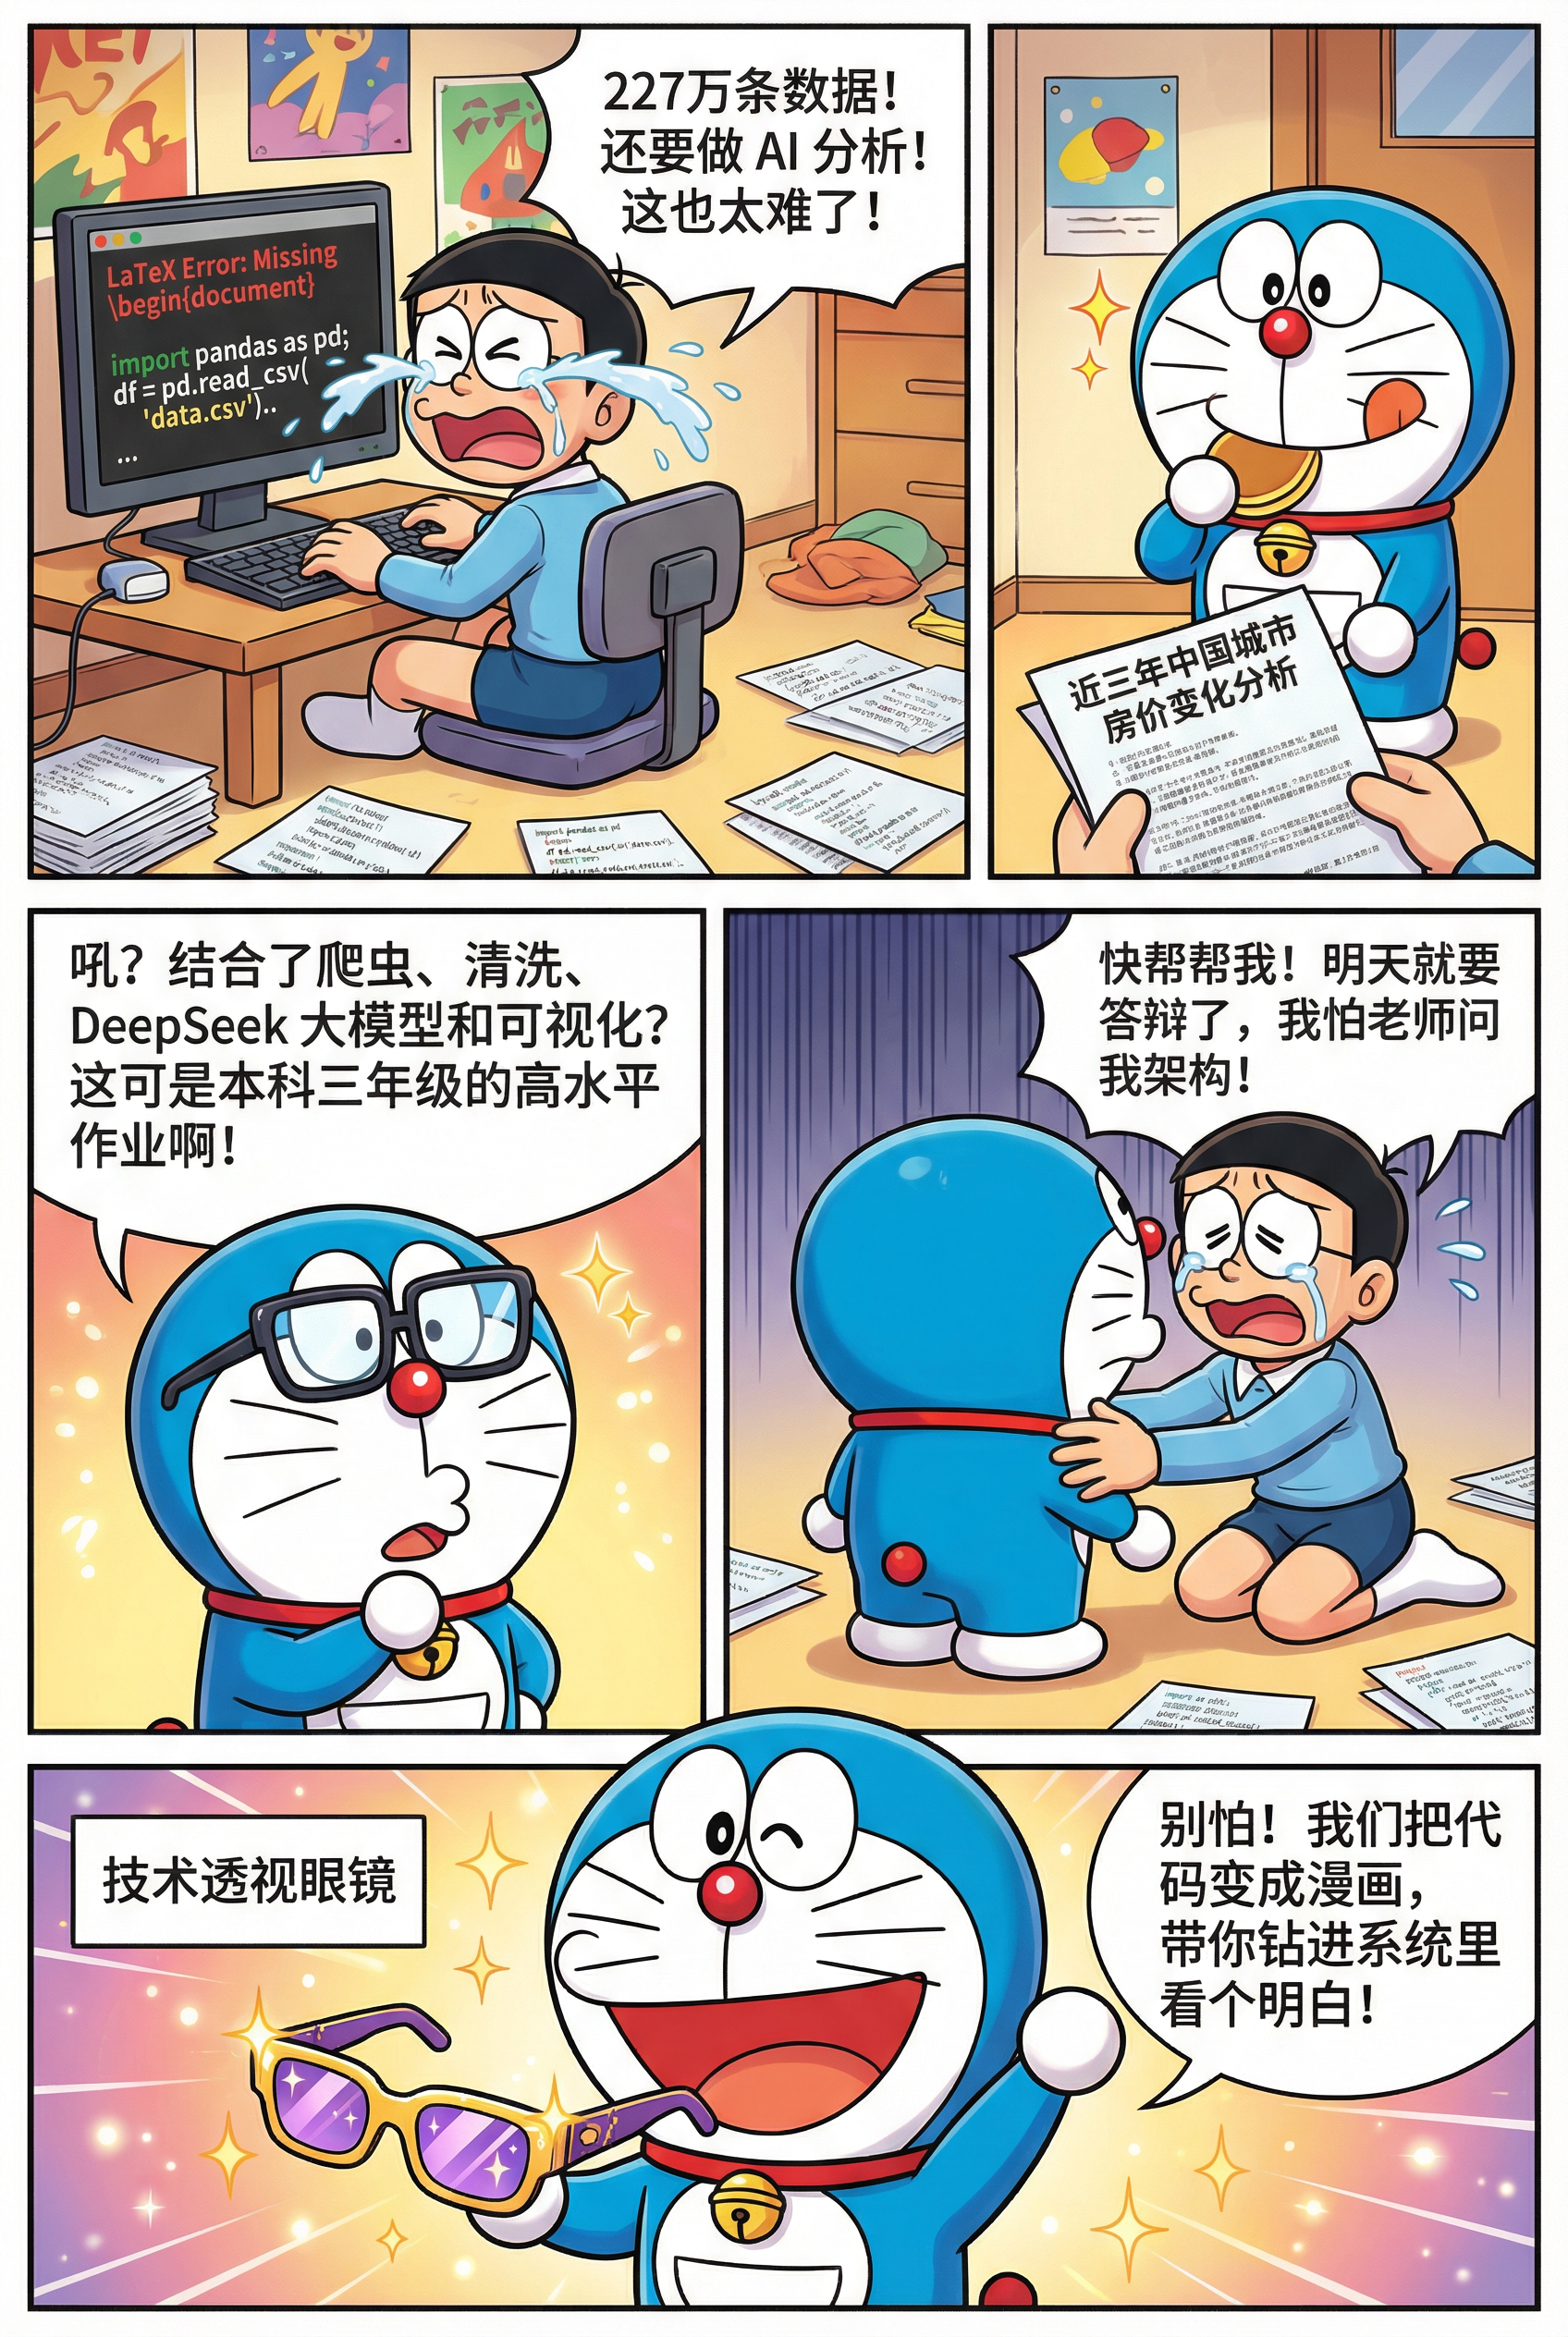
\includegraphics[width=0.85\textwidth]{figures/学习漫画第1页-序章崩溃的大雄与论文危机-彩色版.png}
\caption{第1页:序章——崩溃的大雄与论文危机}
\label{fig:comic1}
\end{figure}

\begin{figure}[H]
\centering

\includegraphics[width=0.85\textwidth]{figures/学习漫画第2页-数据采集隐形斗篷与迷你哆啦.png}
\caption{第2页:数据采集——隐形斗篷与迷你哆啦}
\label{fig:comic2}
\end{figure}

\begin{figure}[H]
\centering

\includegraphics[width=0.85\textwidth]{figures/学习漫画第3页-数据清洗-时光包袱皮的妙用.png}
\caption{第3页:数据清洗——时光包袱皮的妙用}
\label{fig:comic3}
\end{figure}

\begin{figure}[H]
\centering
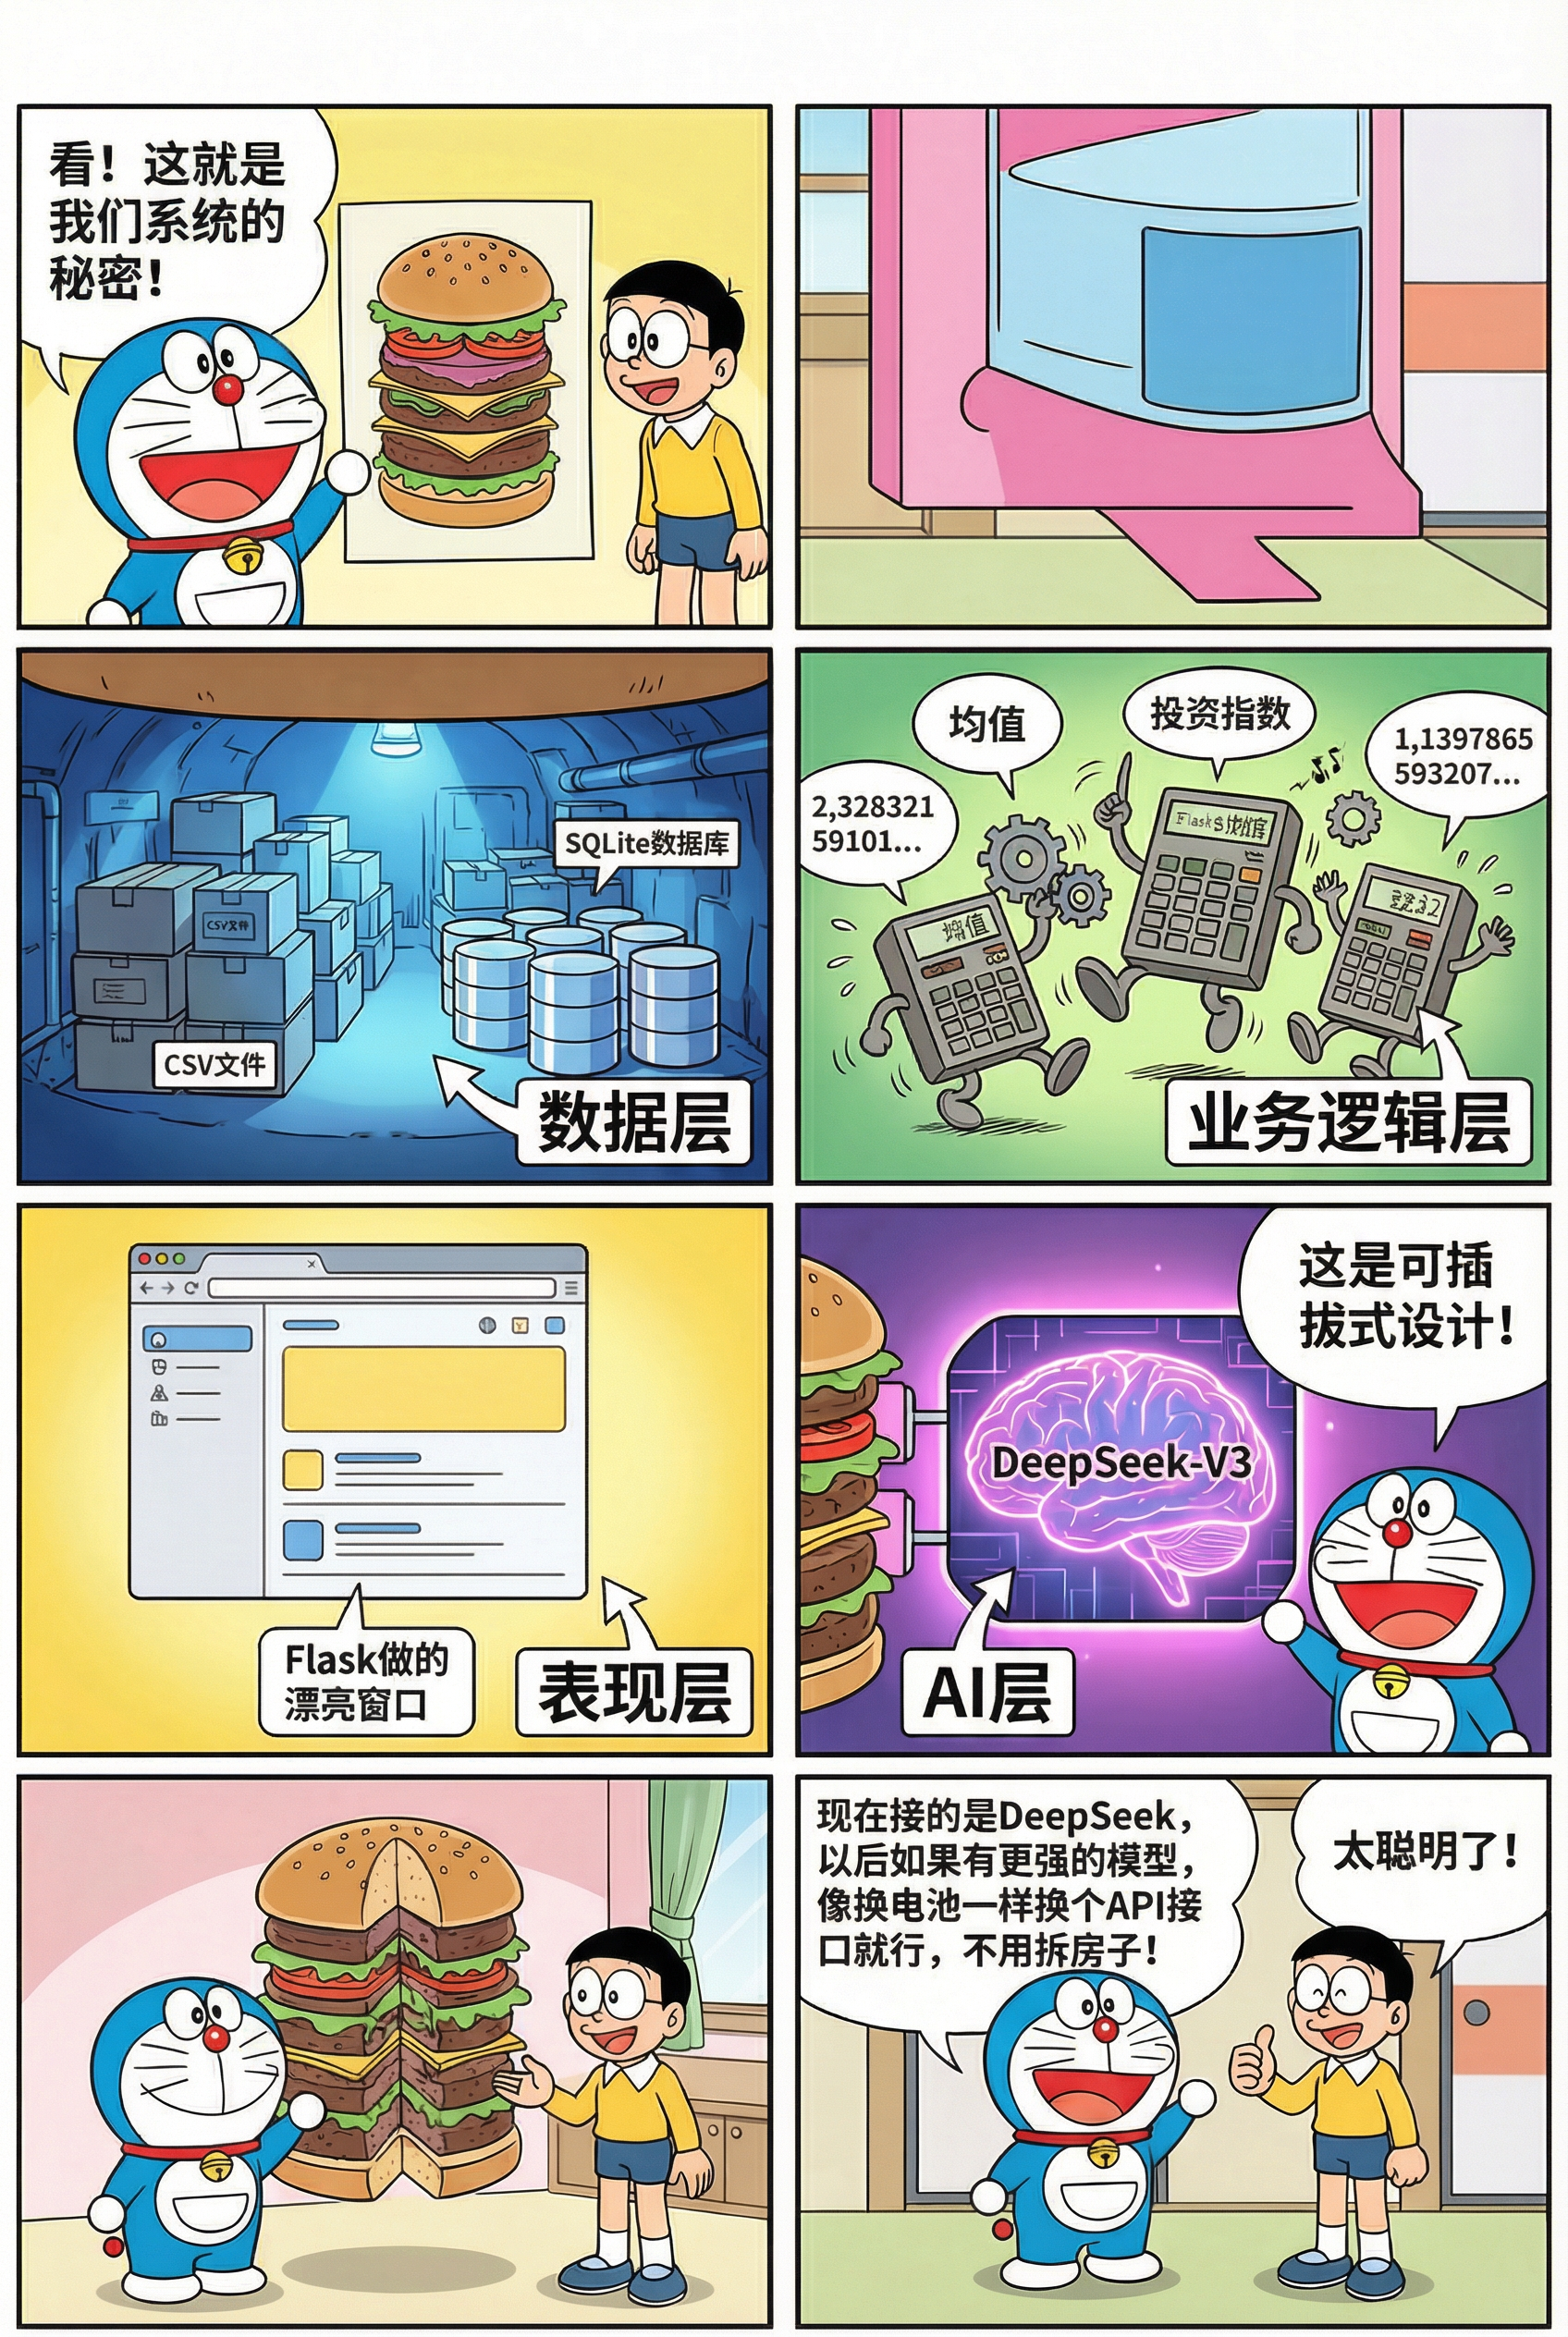
\includegraphics[width=0.85\textwidth]{figures/学习漫画第4页.png}
\caption{第4页:系统分层架构与模块化设计}
\label{fig:comic4}
\end{figure}

\begin{figure}[H]
\centering

\includegraphics[width=0.85\textwidth]{figures/学习漫画第五页-千人千面的身份徽章.png}
\caption{第5页:千人千面的身份徽章(角色个性化系统)}
\label{fig:comic5}
\end{figure}

\begin{figure}[H]
\centering
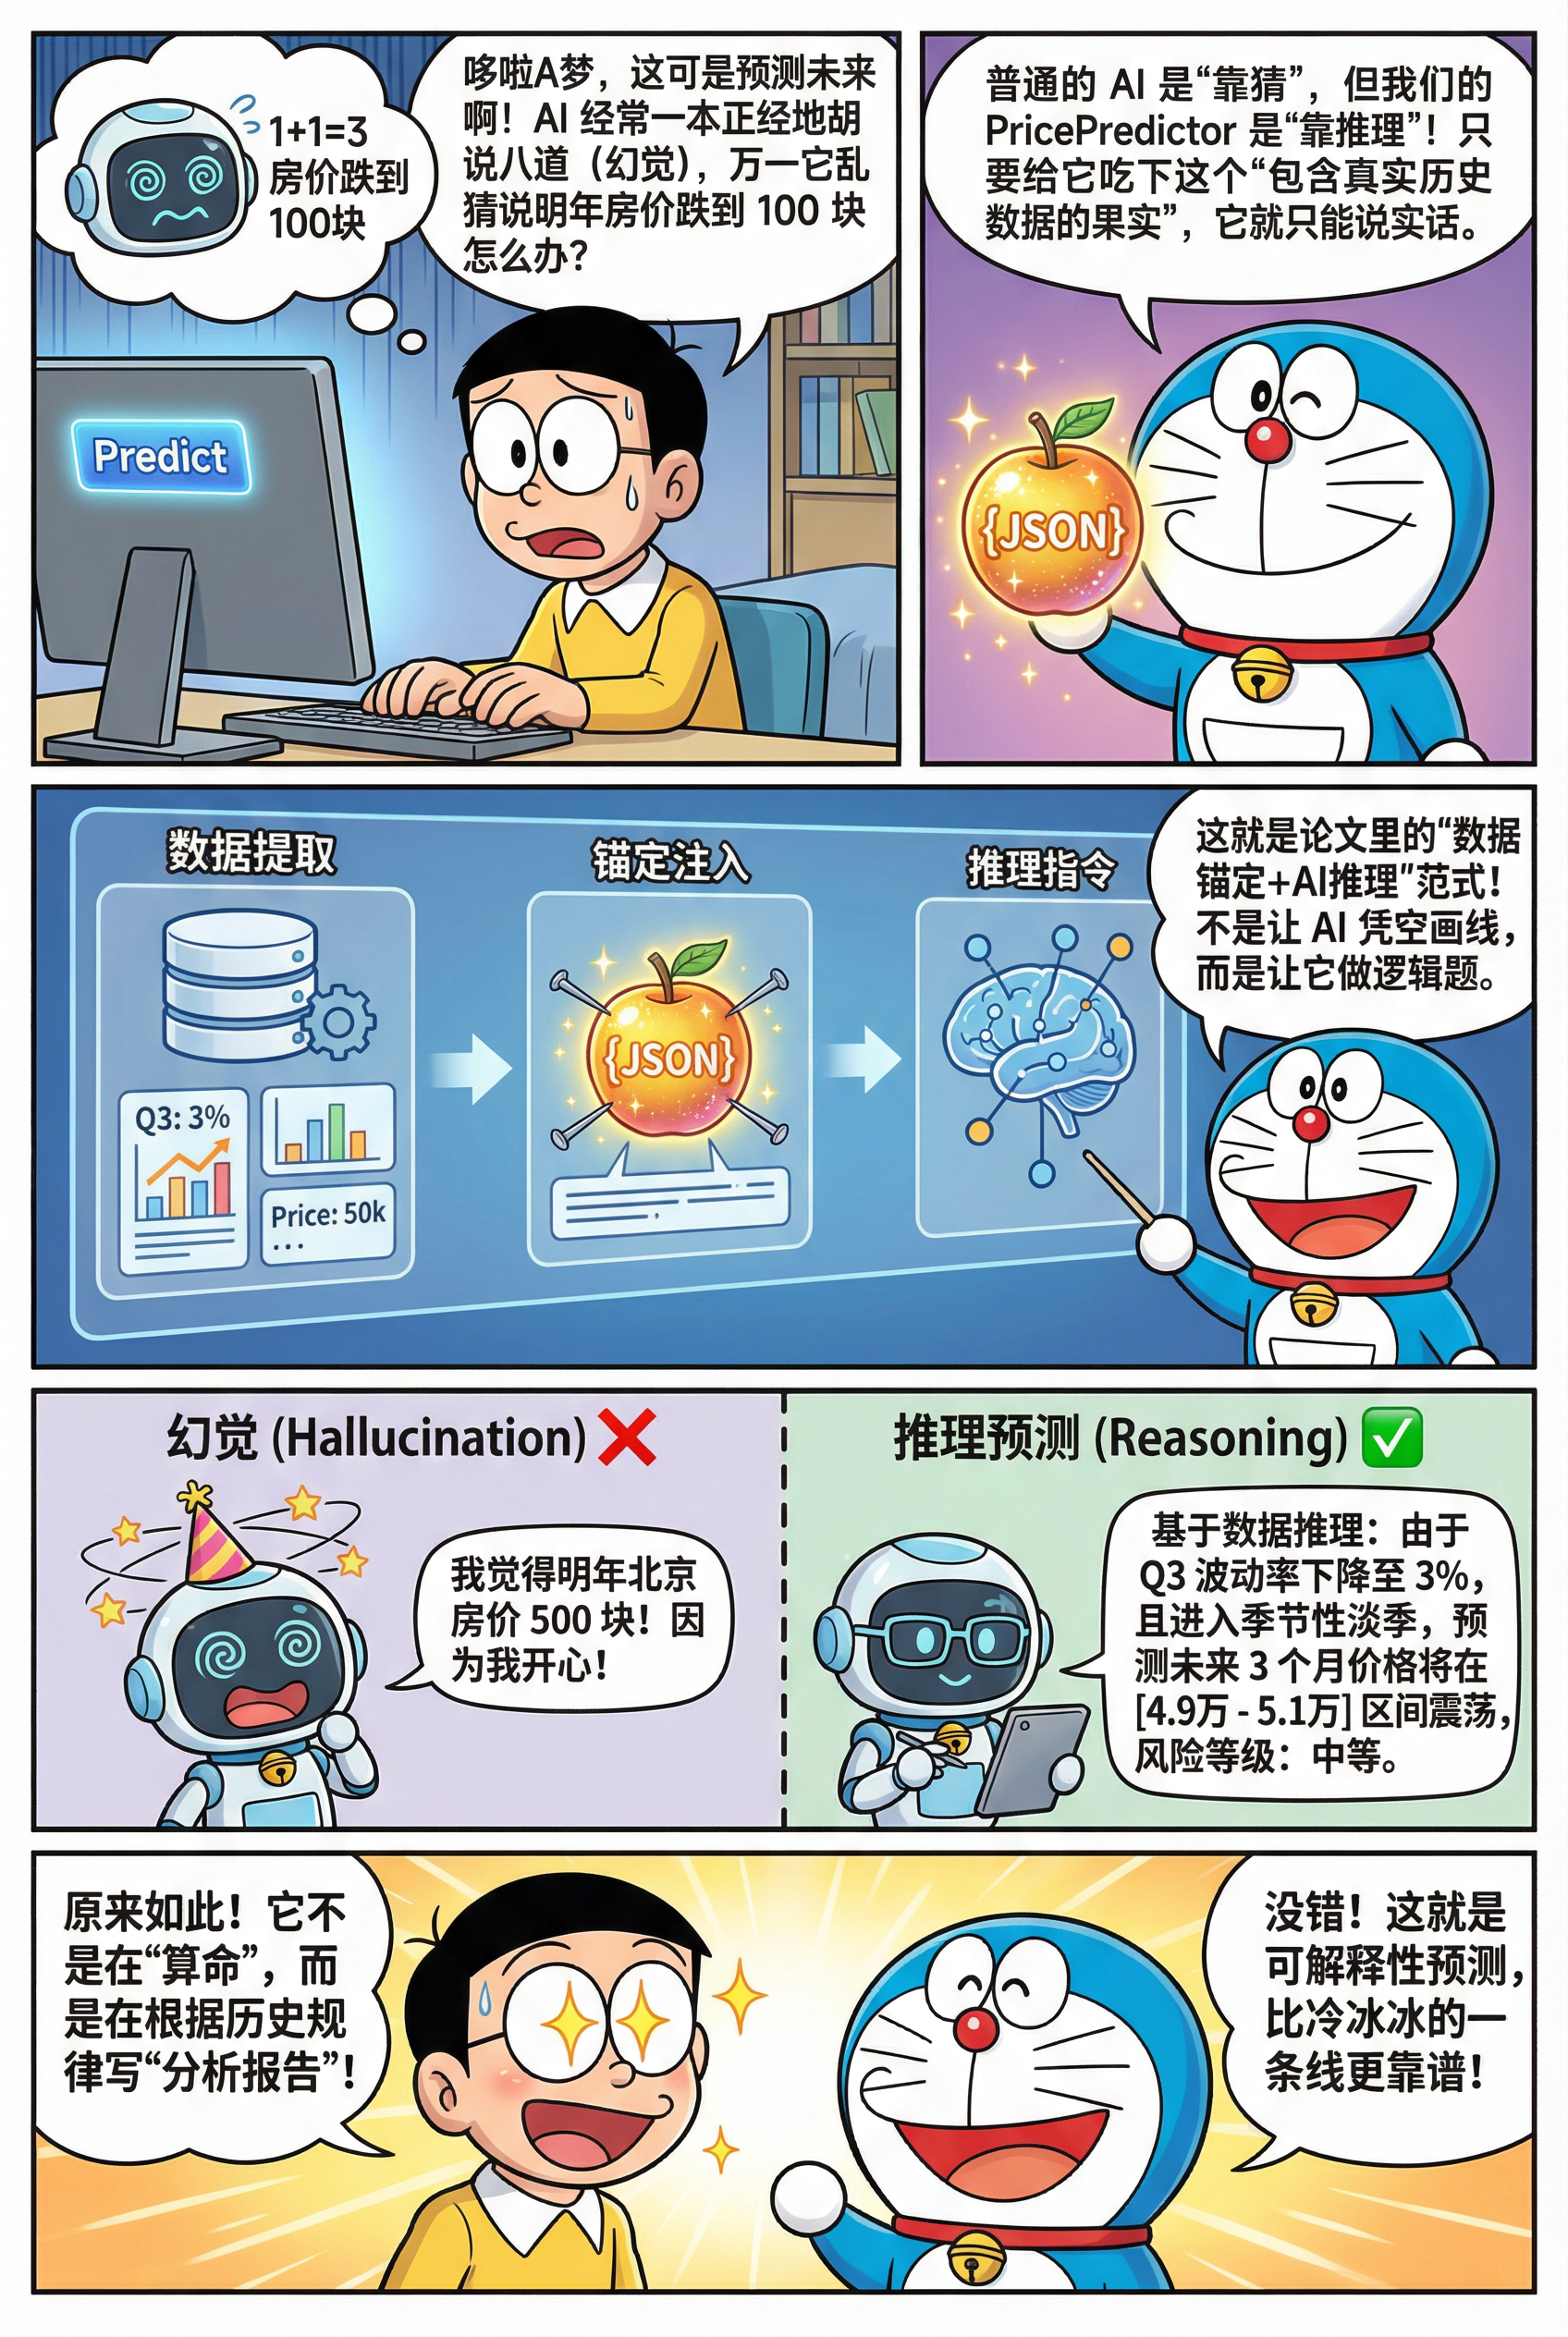
\includegraphics[width=0.85\textwidth]{figures/学习漫画第六页-诚实果实与AI预测引擎.png}
\caption{第6页:诚实果实与AI预测引擎}
\label{fig:comic6}
\end{figure}

\begin{figure}[H]
\centering
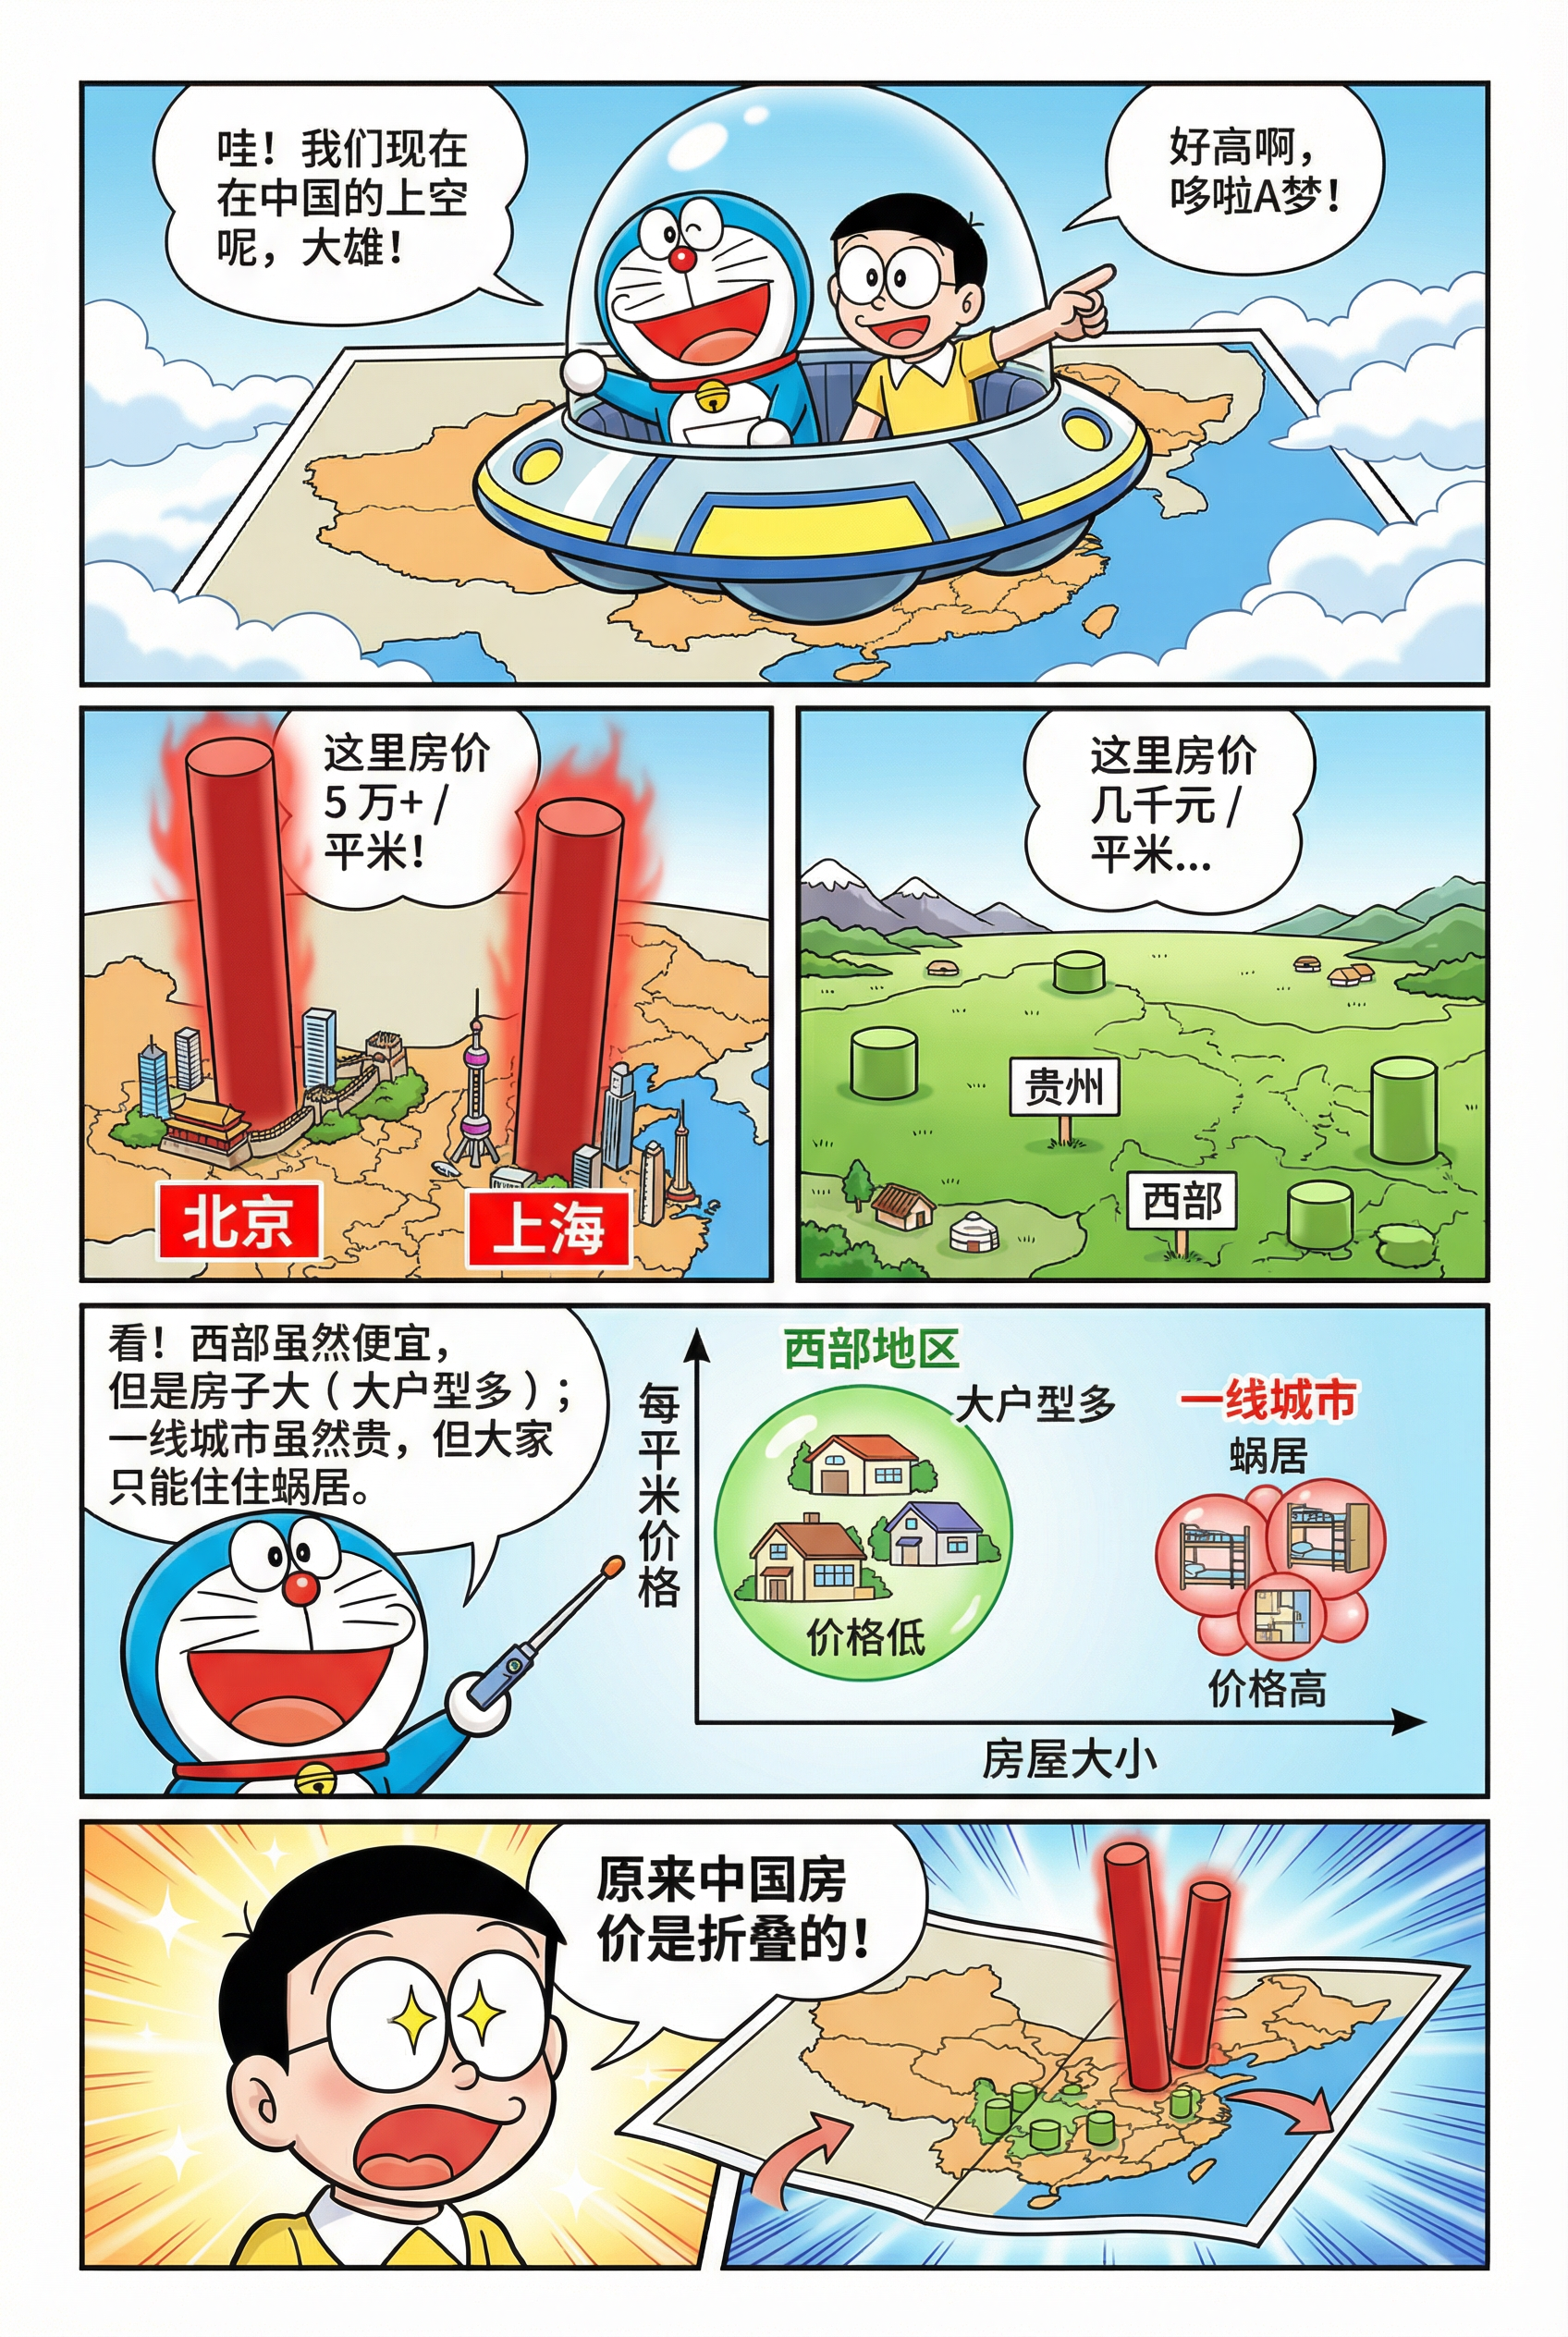
\includegraphics[width=0.85\textwidth]{figures/学习漫画第七页-折叠的中国地图.png}
\caption{第7页:折叠的中国地图(全国房价可视化)}
\label{fig:comic7}
\end{figure}

\begin{figure}[H]
\centering
\includegraphics[width=0.85\textwidth]{figures/学习漫画第八页-过山车与投资公式.png}
\caption{第8页:过山车与投资公式}
\label{fig:comic8}
\end{figure}

\begin{figure}[H]
\centering
\includegraphics[width=0.85\textwidth]{figures/学习漫画第九页-工程伦理与正直太郎.png}
\caption{第9页:工程伦理与正直太郎}
\label{fig:comic9}
\end{figure}

\begin{figure}[H]
\centering
\includegraphics[width=0.85\textwidth]{figures/学习漫画第十页-答辩必胜与未来展望.png}
\caption{第10页:答辩必胜与未来展望}
\label{fig:comic10}
\end{figure}

\end{document}
